\chapter{Tema Principal : Particionamento de malhas \textit{a Priori} para geração em Paralelo de Malhas}\label{tema1}

Nesse capítulo é apresentada a técnica \textit{a priori} proposta de subdivisão de domínios para geração de malhas. Ela foi projetada para atender a alguns requisitos:

\begin{enumerate}
	\item Respeitar a fronteira/superfície de entrada, não realizando nenhuma modificação na mesma;
	
	\item Produzir bons elementos, evitando-se elementos com proporções ruins;
	
	\item Proporcionar boas transições entre as regiões muito refinadas, com muitos elementos pequenos, e regiões grosseiras, com poucos elementos grandes, da malha;
	
	\item Manter a compatibilidade das interfaces dos subdomínios criados com as de seus vizinhos;
	
	\item Abstrair a técnica de geração de malha, podendo-se combinar mais de uma técnica; e
	
	%\item Abstrair o tipo de arquitetura de memória a ser usada (compartilhada ou distribuída); e
	
	\item Tentar gerar malhas da forma mais eficiente possível em termos de tempo de processamento.
\end{enumerate}


O primeiro requisito é muito importante em muitos problemas, tais como aqueles encontrados nas simulações em que o domínio contém regiões com diferentes materiais e/ou buracos. Nesses problemas, geralmente é desejável que a malha esteja em conformidade com uma discretização de contorno já existente nessas regiões.

A técnica proposta utiliza um particionamento contínuo \textit{a priori} que necessita da geração de uma interface interna ao modelo de entrada. A criação desta interface é feita visando a melhor qualidade possível dos elementos que serão gerados, satisfazendo assim o segundo requisito.

Com relação ao terceiro requisito, em muitas aplicações, a diferença de tamanho entre os elementos em uma região refinada e aqueles de uma região grosseira é maior do que duas ordens de magnitude. Assim, para se obter uma boa transição deve-se evitar uma diferença de magnitude maior do que dois.

De acordo com o quarto requisito, é necessário manter a conformidade da malha assim como facilitar a junção da malha de cada partição para obter a malha final. Para isso acontecer é necessário que a malha de interface gerada em um subdomínio tenha a sua simétrica gerada em seu vizinho, isso garante que a malha que será gerada nos dois lados serão compatíveis quando for feita a junção das malhas geradas em cada partição.

O quinto requisito diz que a técnica proposta abstrai o tipo de malha e o gerador que será utilizado, contanto que respeite todos os pré-requisitos aqui citados. Isso permite que possam ser combinadas diferentes técnicas de geração de malha, como as de Delaunay e Avanço de Fronteira, por exemplo.

O último requisito é também muito importante, já que a velocidade e a qualidade da malha são atualmente um dos principais objetivos de estudo na área da geometria computacional.

É importante observar que, apesar destes trabalho focar na geração de malhas tridimensionais, a técnica paralela é genérica, e funciona tanto para duas quanto para três dimensões. Assim, sempre que for mais didático, o caso bidimensional será utilizado para exemplificar alguns aspectos da técnica.



\section{Algoritmo \textit{a Priori}}

Na técnica proposta a entrada pode ser uma lista de segmentos que definem uma fronteira, para o caso bidimensional, ou um conjunto de faces que definem uma superfície, para o caso tridimensional. A entrada pode definir um ou mais objetos, que podem conter ou não buracos. 

Uma estrutura de dados do tipo árvore(\textit{quadtree} para o caso bidimensional e \textit{octree} para o caso tridimensional) será criada e refinada de acordo com o tamanho dos elementos dados como entrada(arestas para o caso bidimensional e faces para o caso tridimensional), levando em consideração que o tamanho das células internas desta árvore não pode ser maior que o maior elemento da entrada. Esta estrutura de dados é chamada de \textit{quadtree} ou \textit{octree} de densidade ou de carga.

Com a árvore de densidade devidamente criada, a estimativa de carga é realizada. Este processo de estimativa é feito baseado na quantidade de células que são internas ao domínio. O próximo passo é o particionamento da entrada em diversas partes. Para realizar o particionamento do domínio, uma estrutura de dados espacial que divide regiões nos eixos cartesianos deve ser utilizada para que a técnica de geração de subdomínios funcione perfeitamente. Isso será mostrado na seção \ref{sec:Decomposicao_dominio}.

O algoritmo de geração das malhas de interfaces dos subdomínios recebe o resultado do particionamento do domínio e cria os novos subdomínios, tendo cada um deles sua interface totalmente compatível com as de seus vizinhos.

Após a criação de todos subdomínios, o balanceamento de carga é feito caso o número de processos criados seja maior que a quantidade de processadores disponíveis para executar a geração da malha. A malha é então gerada em cada um dos subdomínios e ao final é feita uma junção dos pedaços da malha e realizado algumas melhorias. A Figura \ref{fig:fluxograma} mostra o fluxograma de como a técnica procede.

\begin{figure}[!ht]
	\centering
	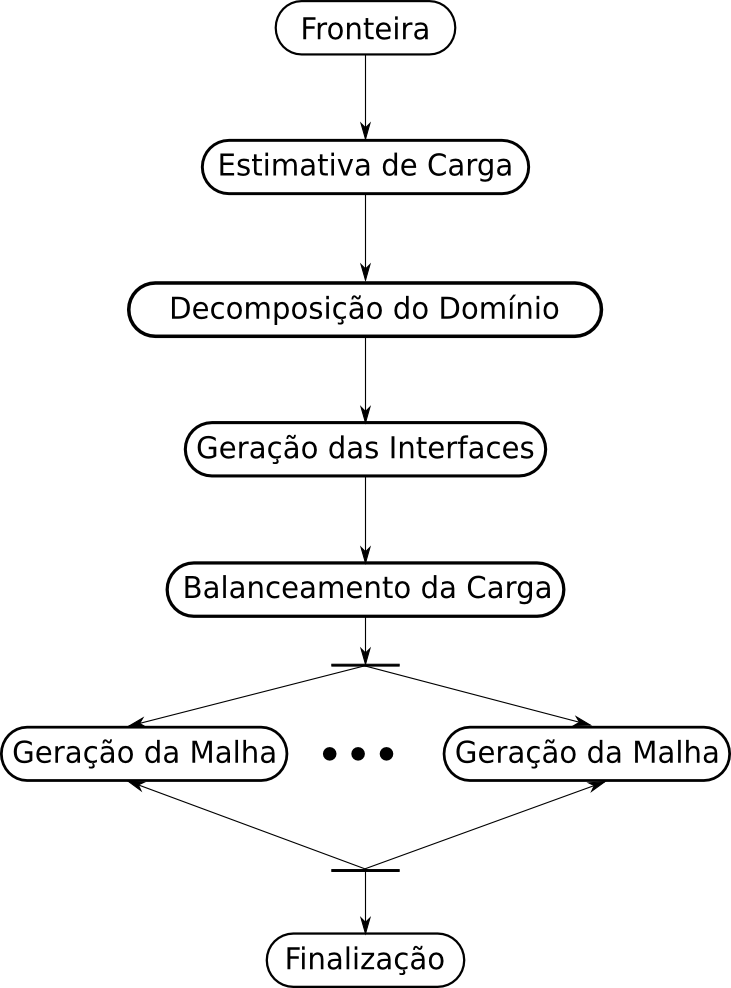
\includegraphics[width=0.6\textwidth]{fig/fluxograma.png}
	\caption{Visão geral da técnica paralela.}
	\label{fig:fluxograma}
\end{figure}


\section{Estimativa de Carga} 
\label{sec:Estimativa_de_Carga}

Em Computação de Alto Desempenho (CAD), a carga é uma medida da quantidade de trabalho a ser realizado em um subdomínio ou um conjunto de subdomínios. Em problemas de geração de malha, a carga está relacionada com o número de elementos que serão gerados em cada subdomínio. Portanto, a carga está relacionada com as seguintes questões, que devem ser levadas em conta em sua estimativa (Figuras~\ref{fig:malha_norma_refinada} e~\ref{fig:malha_uniforme_não_uniforme}):

\begin{itemize}
	\item O nível de discretização da malha, geralmente especificado pelo usuário ou por outro software, através de parâmetros de entrada. Quanto maior a discretização da malha, maior será a carga (Figura \ref{fig:malha_norma_refinada} e \ref{fig:malha_norma_refinada_trid}).

\begin{figure}[!ht]
	\centering
	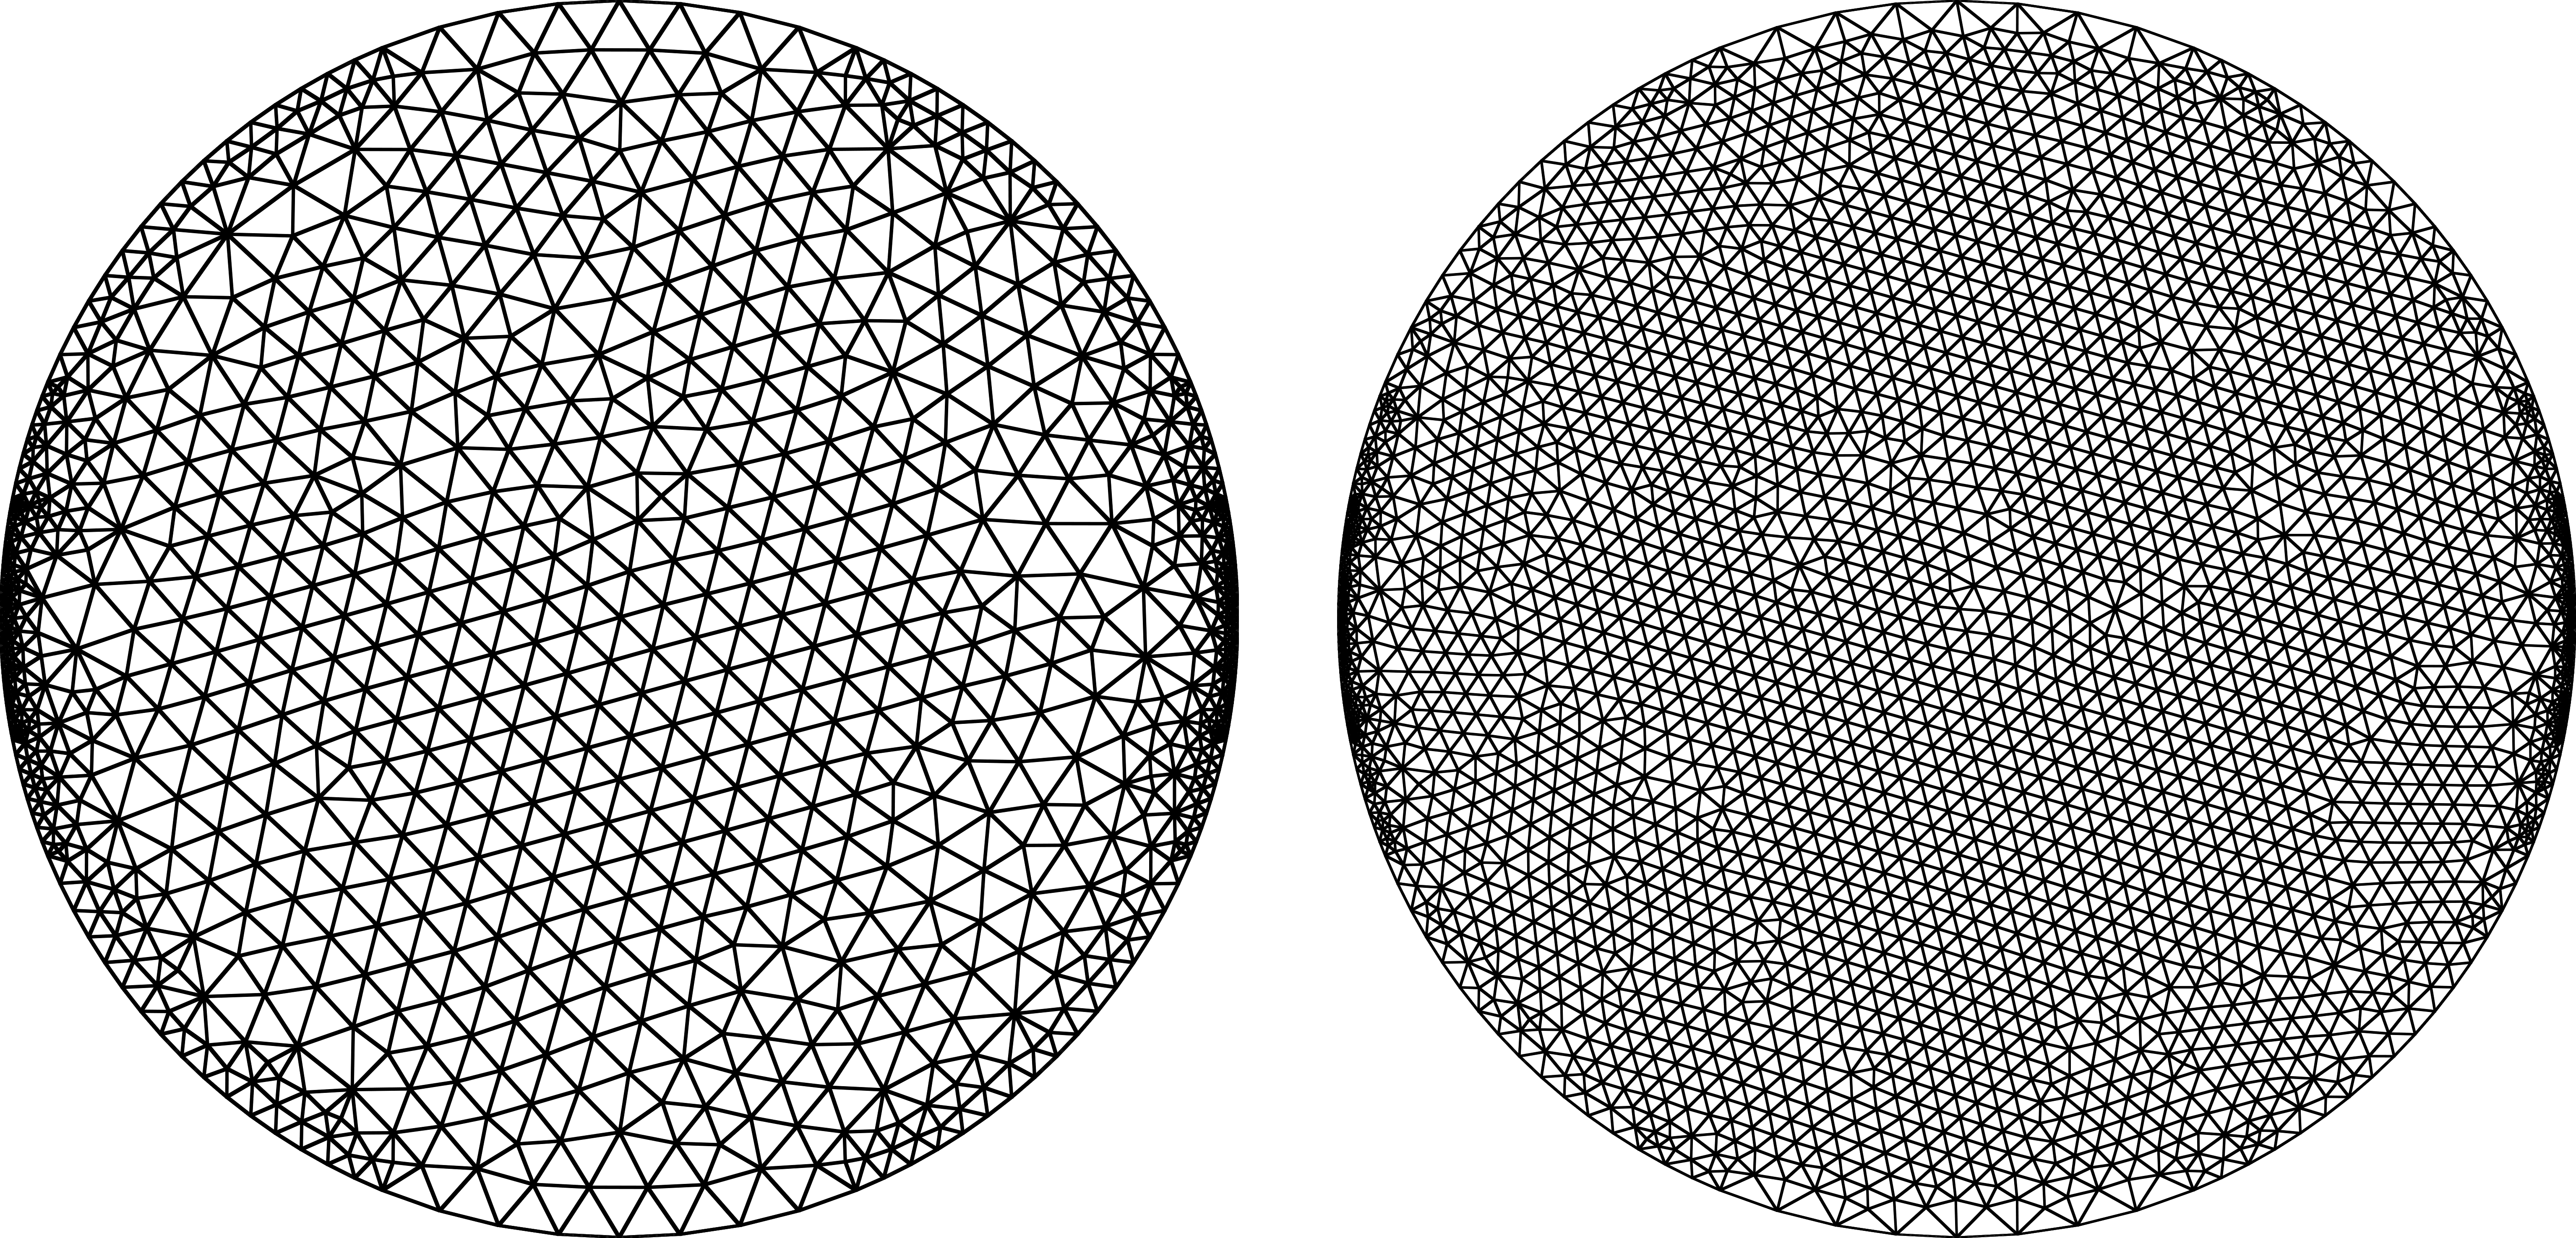
\includegraphics[width=1.0\textwidth]{fig/meshes_normal_and_refined.png}
	\caption{Estimativa de carga para o caso bidimensional: refinamento menor (esquerda) e maior (direita).}
	\label{fig:malha_norma_refinada}
\end{figure}

\begin{figure}[!ht]
	\centering
	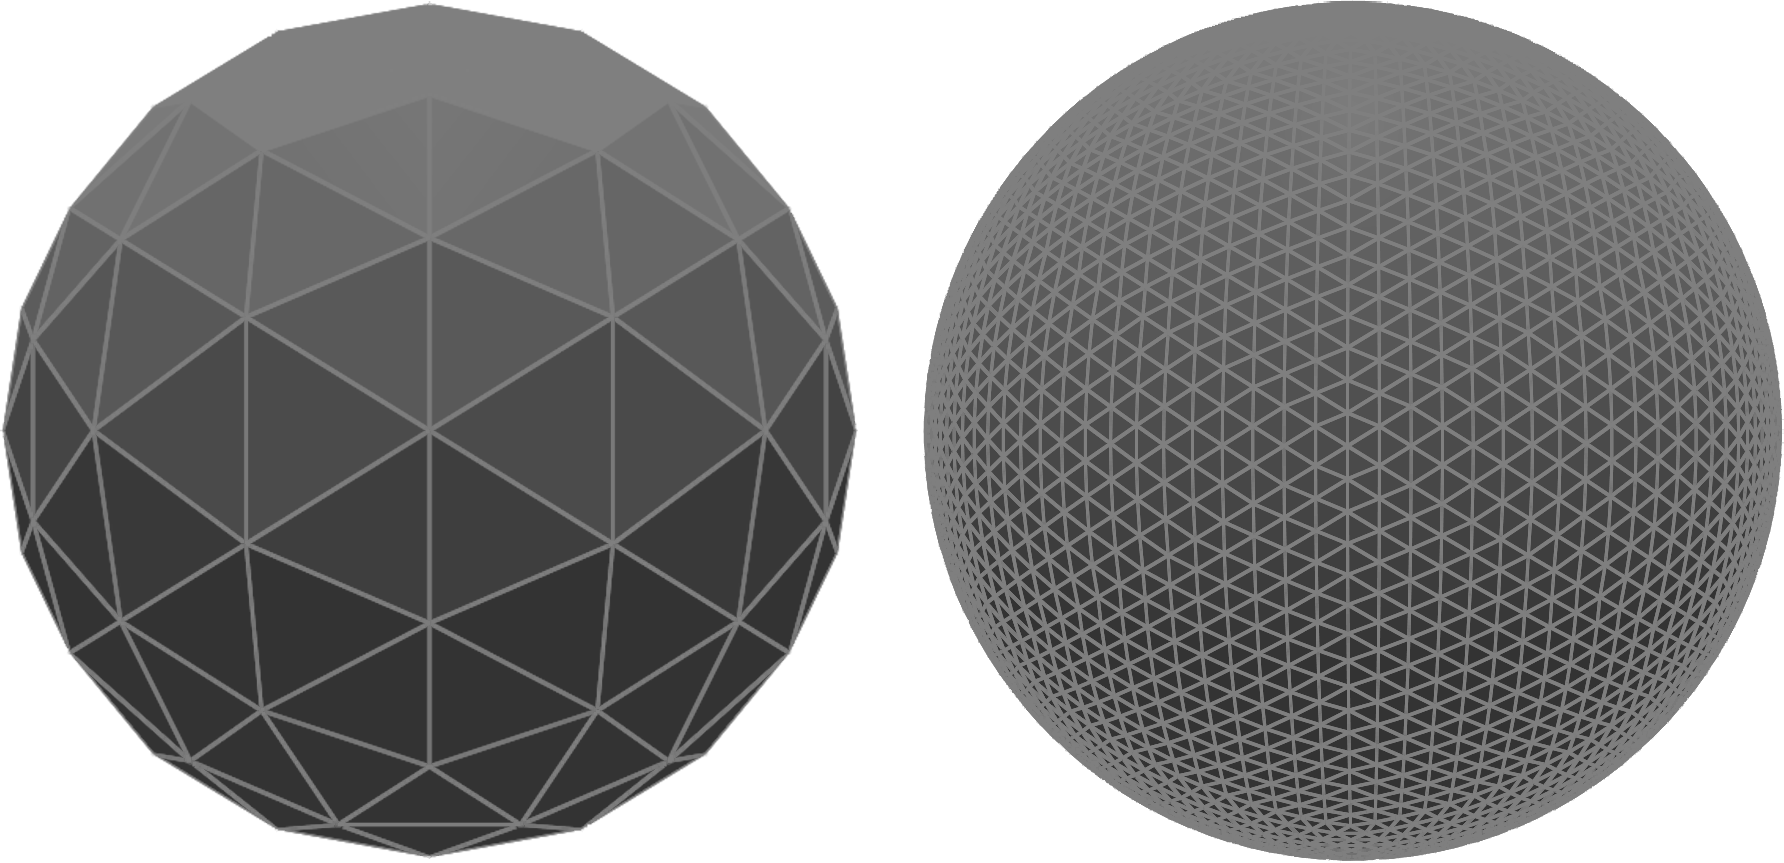
\includegraphics[width=1.0\textwidth]{fig/esferas_comp_ref.png}
	\caption{Estimativa de carga para o caso tridimensional: refinamento menor (esquerda) e maior (direita).}
	\label{fig:malha_norma_refinada_trid}
\end{figure}

	\item Em regiões com o mesmo nível de discretização, uma região maior gera mais elementos do que uma região menor. Assim, quanto maior for a região, maior será a carga (esquerda da Figura \ref{fig:malha_uniforme_não_uniforme} e \ref{fig:malha_uniforme_não_uniforme_trid}).
	\item Em domínios com diferentes níveis de discretização, regiões de mesmo tamanho podem gerar um número de elementos diferente, dependendo do nível de refinamento de cada região. Assim, quanto mais refinada for a malha na região, maior será a carga(direita da Figura \ref{fig:malha_uniforme_não_uniforme} e \ref{fig:malha_uniforme_não_uniforme_trid}).
\end{itemize}


\begin{figure}[!ht]
	\centering
	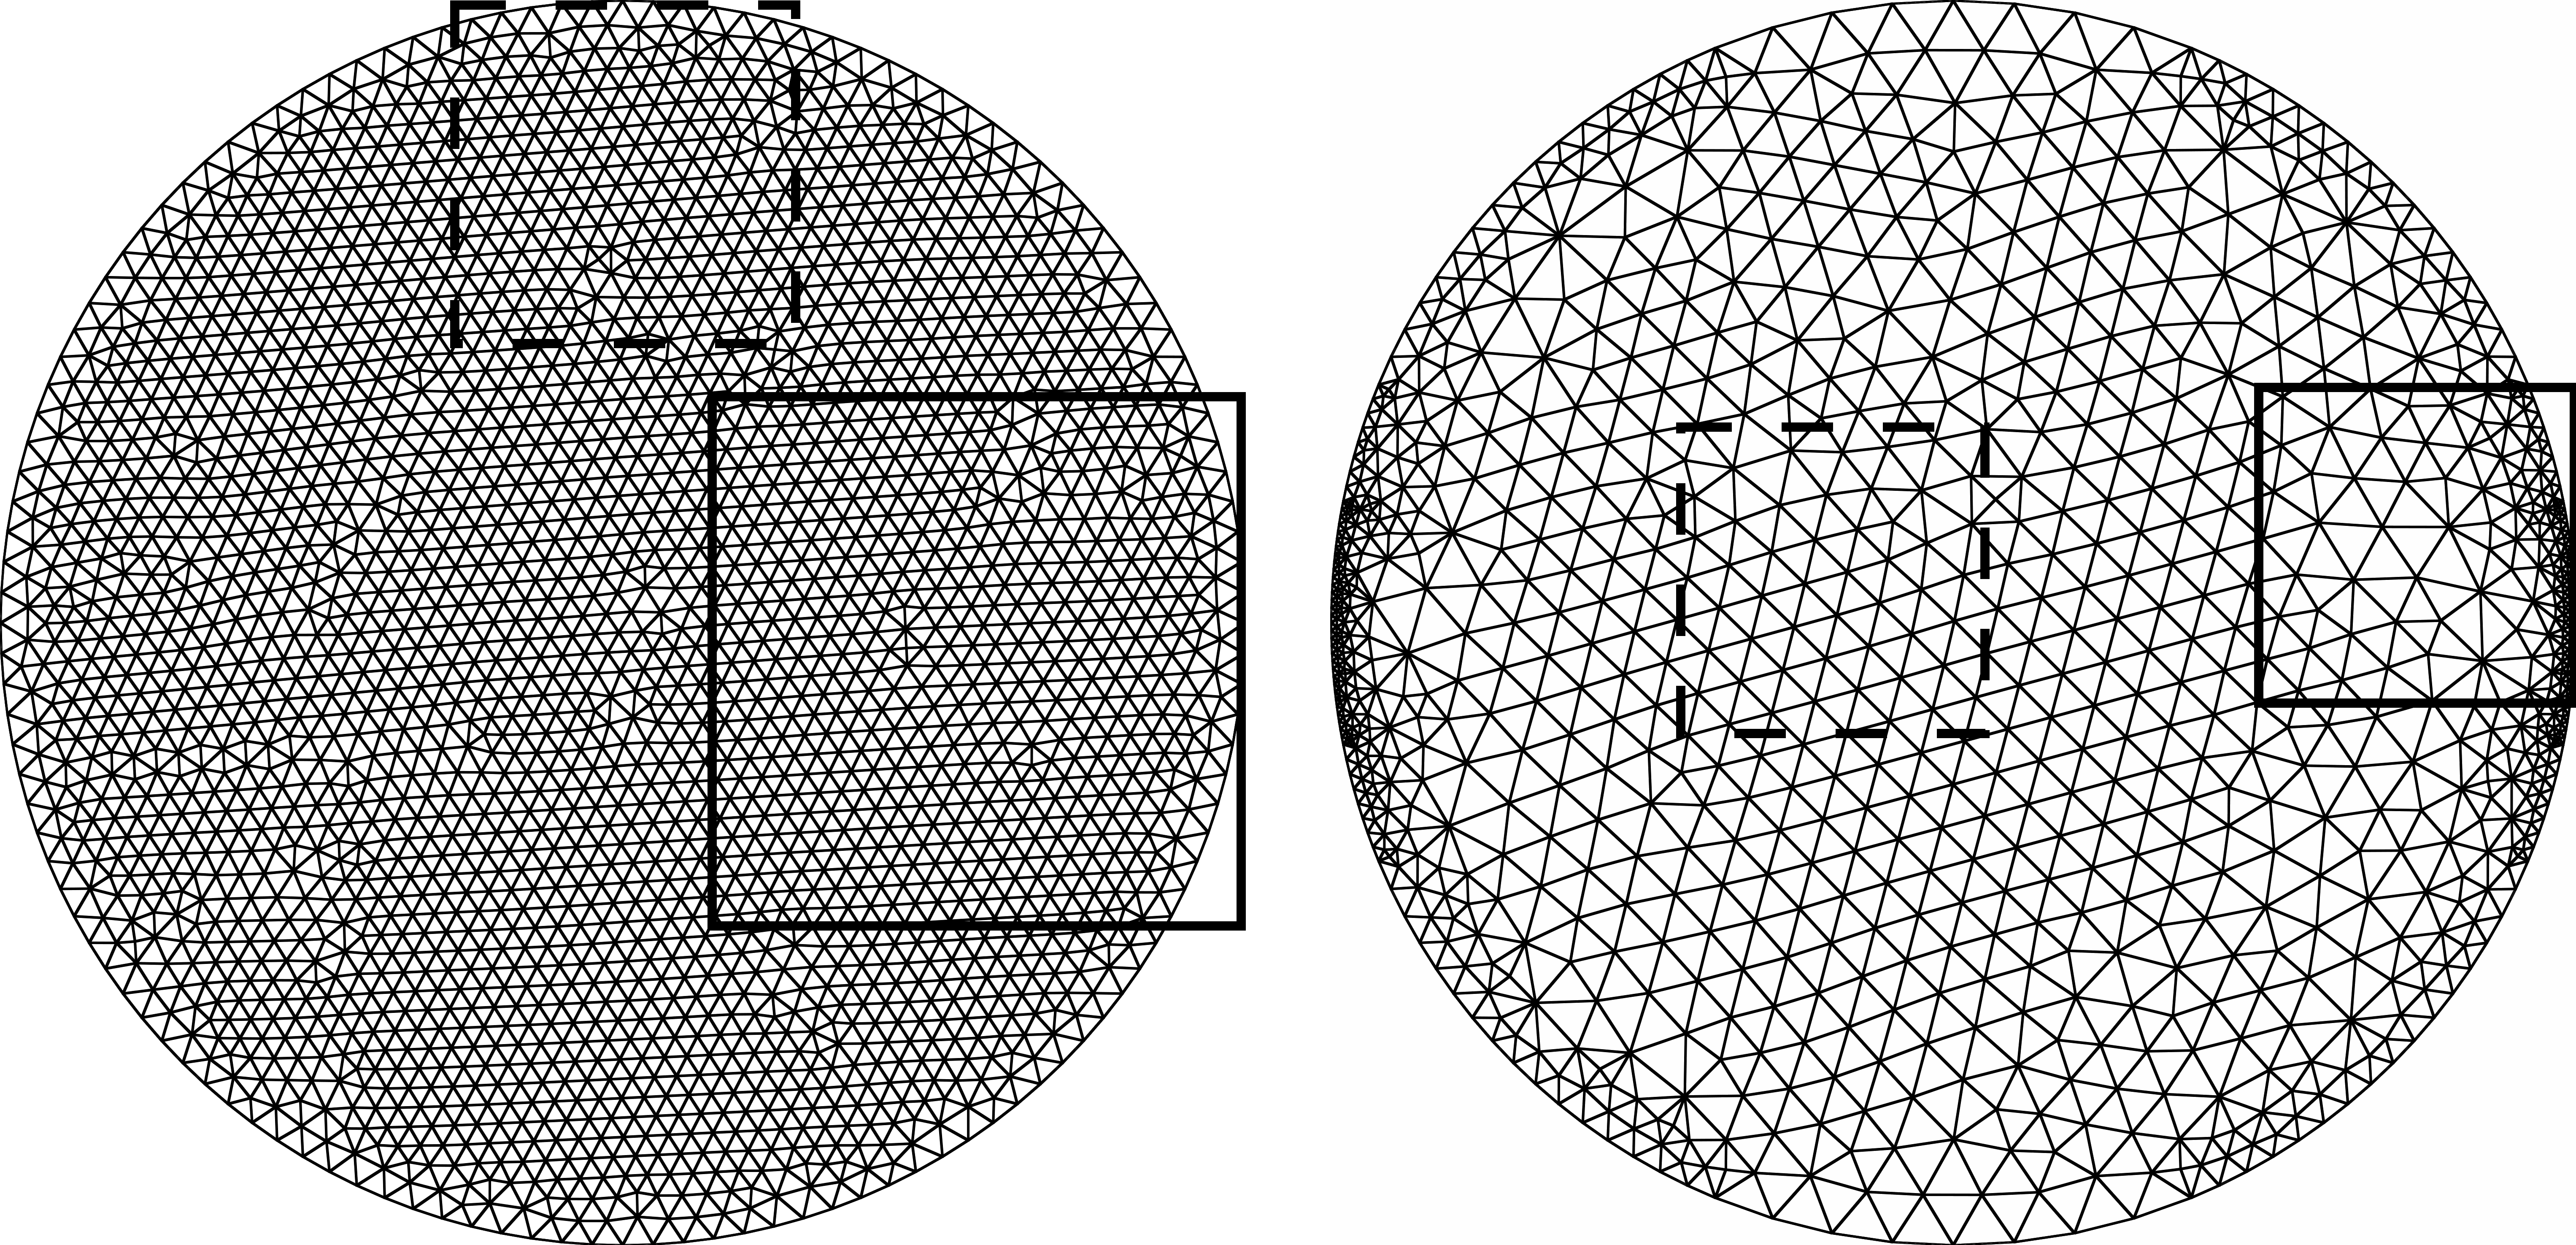
\includegraphics[width=1.0\textwidth]{fig/meshes_transition_and_uniform.png}
	\caption{Estimativa de carga para o caso bidimensional: malha uniforme (esquerda) e não-uniforme (direita).}
	\label{fig:malha_uniforme_não_uniforme}
\end{figure}

\begin{figure}[!ht]
	\centering
	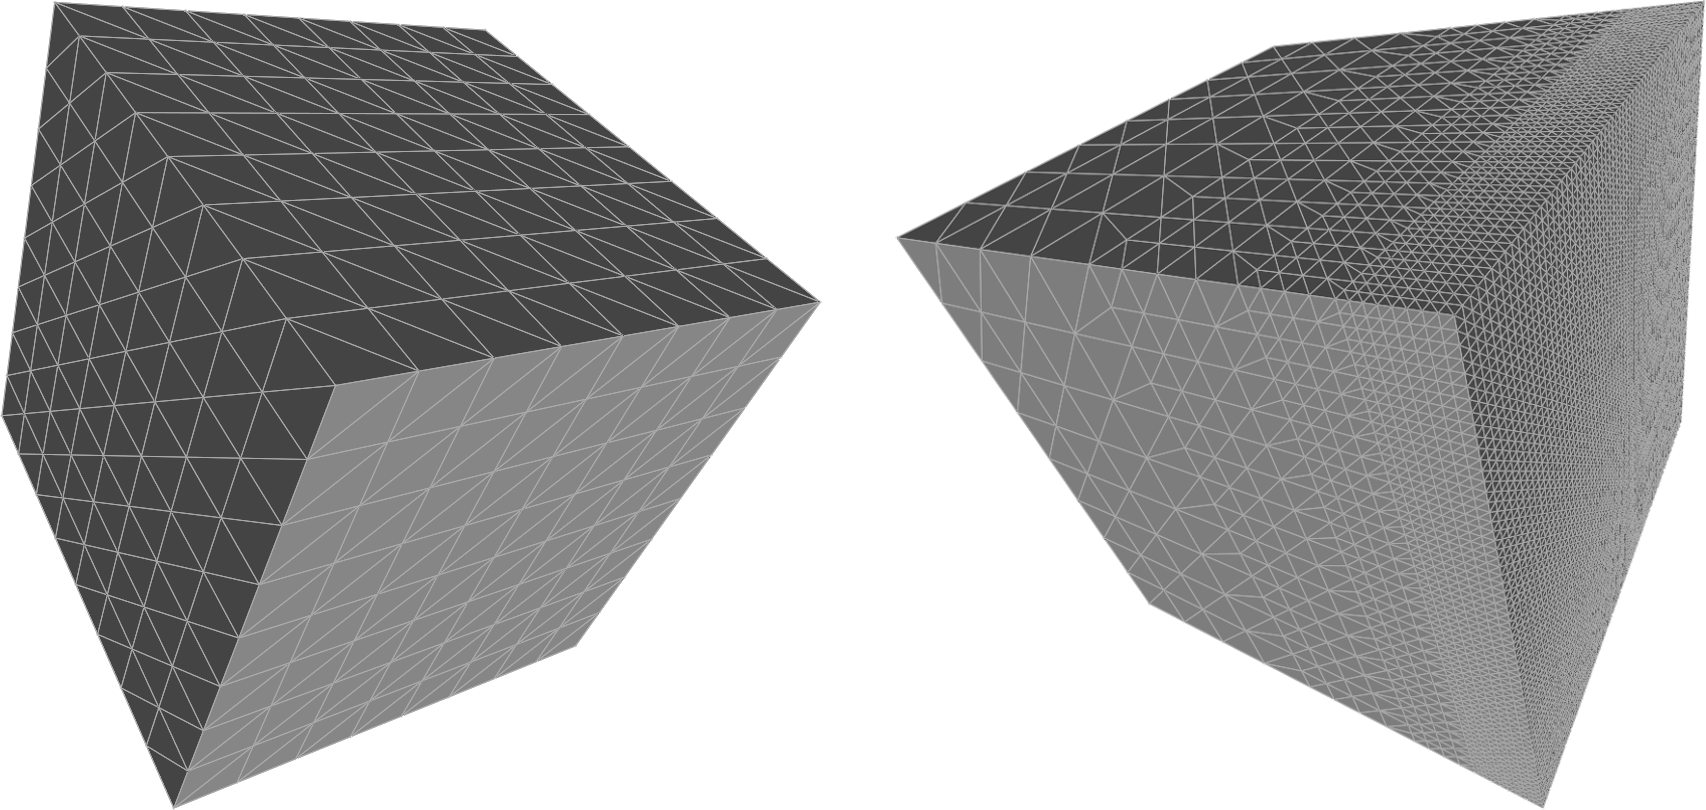
\includegraphics[width=1.0\textwidth]{fig/cubes_comp_uniform.png}
	\caption{Estimativa de carga para o caso tridimensional: face de um cubo com malha uniforme (esquerda) e uma face de um cubo com malha não-uniforme (direita).}
	\label{fig:malha_uniforme_não_uniforme_trid}
\end{figure}

A malha da direita da Figura~\ref{fig:malha_norma_refinada} sugere uma carga maior que a malha da esquerda da mesma figura. A mesma discretização de borda foi utilizada nos dois casos. Na Figura~\ref{fig:malha_uniforme_não_uniforme}, a carga associada às regiões cercadas por linhas contínuas é maior que a carga associada às regiões cercadas por linhas tracejadas.

\subsection{Estrutura de Estimativa de Carga}

Para estimar a carga de um modelo dado como entrada é utilizado uma \textit{quadtree}, caso seja bidimensional, ou uma \textit{octree}, caso seja tridimensional. As mesmas regras de criação da \textit{quadtree} se aplicam na \textit{octree}, sendo assim, por ser mais simples de representar e entender, será explicado todo o processo usando como base a \textit{quadtree}.

A \textit{quadtree} de estimativa de carga ou \textit{quadtree} de densidade é utilizada tanto para estimar a carga como para auxiliar a geração das malhas de interface. Sua criação é iniciada com a construção de um quadrado de tamanho mínimo que engloba toda a fronteira dada como entrada (Figura \ref{fig:passo0_estimativa}); este quadrado é a célula-raiz da \textit{quadtree}. Esta \textit{quadtree} será subdividida até que todos os pontos médios das arestas da entrada estejam dentro de uma célula da \textit{quadtree} de densidade (Figura \ref{fig:passo1_estimativa}). O tamanho destas células tem de ser menor que o comprimento da aresta à qual o ponto médio pertence, multiplicada por uma constante. Essa constante tem valor $\sqrt{3}/2$, que equivale a 0,85, que é uma aproximação da altura de um triângulo equilátero. Para o caso tridimensional esta constante tem valor $\sqrt{6}/3$, que equivale a 0,81, que é uma aproximação da altura de um tetraedro regular.

Dois refinamentos são então aplicados. O primeiro é para garantir que todas as células da \textit{quadtree} de densidade não sejam maiores que a maior célula que contém um ponto médio da borda de entrada (Figura \ref{fig:passo2_estimativa}). Com esse refinamento é garantido um tamanho máximo para as células de acordo com as arestas da fronteira. Assim, os elementos que serão gerados no interior do domínio terão proporções iguais aos da borda. 

O segundo refinamento, também conhecido na literatura como refinamento 2:1, é para garantir que a diferença de níveis da \textit{quadtree} não seja maior que 2 para células vizinhas (que compartilham um lado), como mostrado na Figura \ref{fig:passo3_estimativa}. Este refinamento é feito para garantir uma transição suave entre elementos grandes e pequenos. Mais detalhes de como essa \textit{quadtree} é construída podem ser encontrados em~\cite{bib:Miranda99} (a construção de sua versão tridimensional, uma \textit{octree}, pode ser encontrada em~\cite{bib:Cavalcante-Neto01}).


    \begin{figure}[ht]
    	\centering
    	\subfloat[Fronteira de entrada juntamente com sua caixa delimitadora (em vermelho).]
    	{\label{fig:passo0_estimativa}
    		\begin{minipage}[c]{0.4\textwidth}{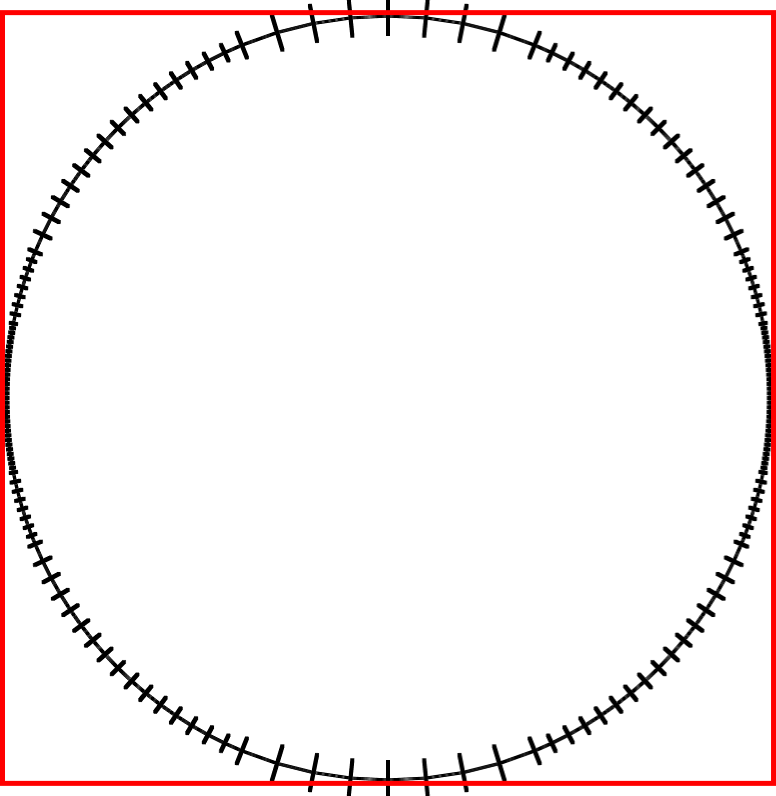
\includegraphics[width=\textwidth]{fig/passo0.png}}\end{minipage}
    	}
    	\qquad
    	\subfloat[\textit{Quadtree} de densidade inicialmente gerada.]
    	{\label{fig:passo1_estimativa}
    		\begin{minipage}[c]{0.4\textwidth}{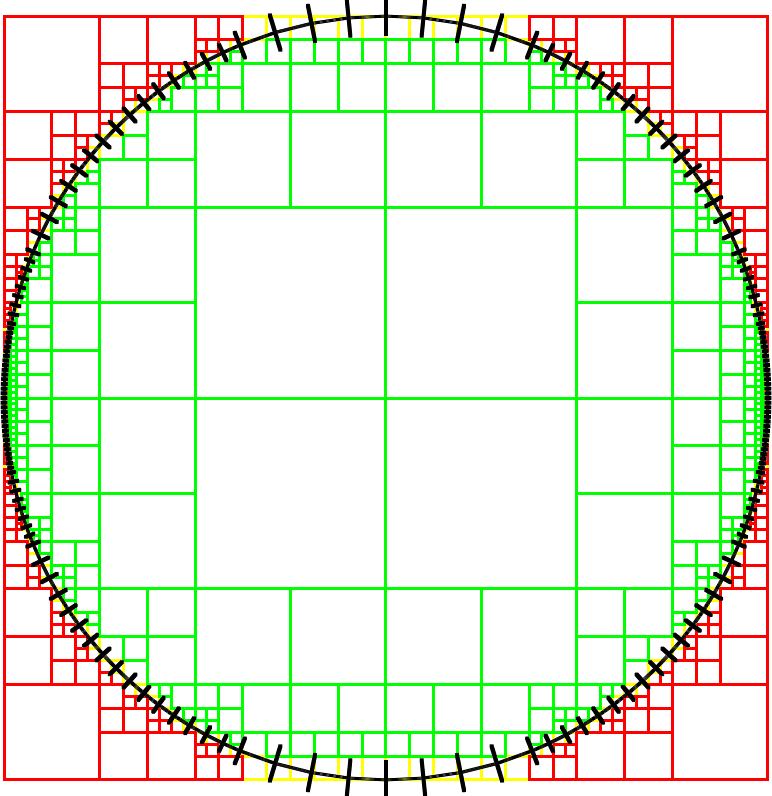
\includegraphics[width=\textwidth]{fig/passo1.png}}\end{minipage}
    	}
    	
    	\subfloat[Primeiro refinamento na \textit{quadtree} de densidade.]
    	{\label{fig:passo2_estimativa}
    		\begin{minipage}[c]{0.4\textwidth}{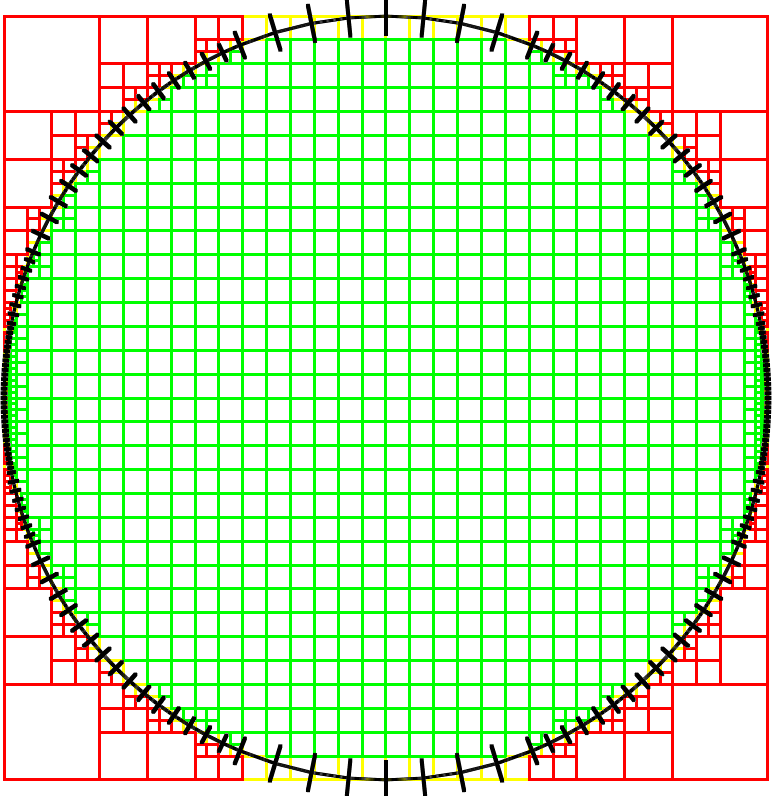
\includegraphics[width=\textwidth]{fig/passo2.png}}\end{minipage}
    	}    
    	\qquad
    	\subfloat[Segundo refinamento na \textit{quadtree} de densidade.]
    	{\label{fig:passo3_estimativa}
    		\begin{minipage}[c]{0.4\textwidth}{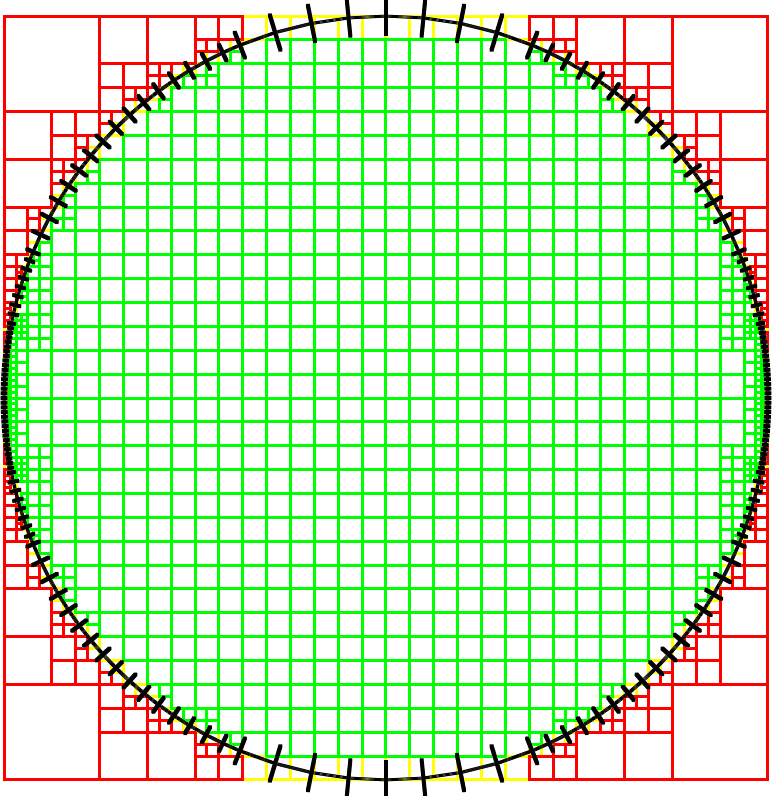
\includegraphics[width=\textwidth]{fig/passo3.png}}\end{minipage}
    	}
    	\caption{Passos da geração da \textit{quadtree} de densidade.}
    	\label{fig:passos_estimativa}
    \end{figure}


\subsection{Classificação das Células}

Uma classificação das células da \textit{quadtree} de densidade contribui para otimizar buscas e para evitar o desperdício de memória. Pode-se classificar uma célula como interna (caso a célula esteja totalmente interna ao domínio), externa (caso a célula esteja totalmente externa ao domínio) ou sobre a fronteira do domínio (caso a célula faça interseção com alguma aresta ou vértice do domínio). O algoritmo de classificação é mostrado em \cite{bib:Freitas10}. A Figura \ref{fig:classificacao} mostra as células de uma \textit{quadtree} de densidade classificadas para um dado domínio circular, onde as cores atribuídas às células indicam a sua classificação (células verdes - dentro do domínio, células vermelhas - fora do domínio, células amarelas - sobre a fronteira).

\begin{figure}[!ht]
	\centering
	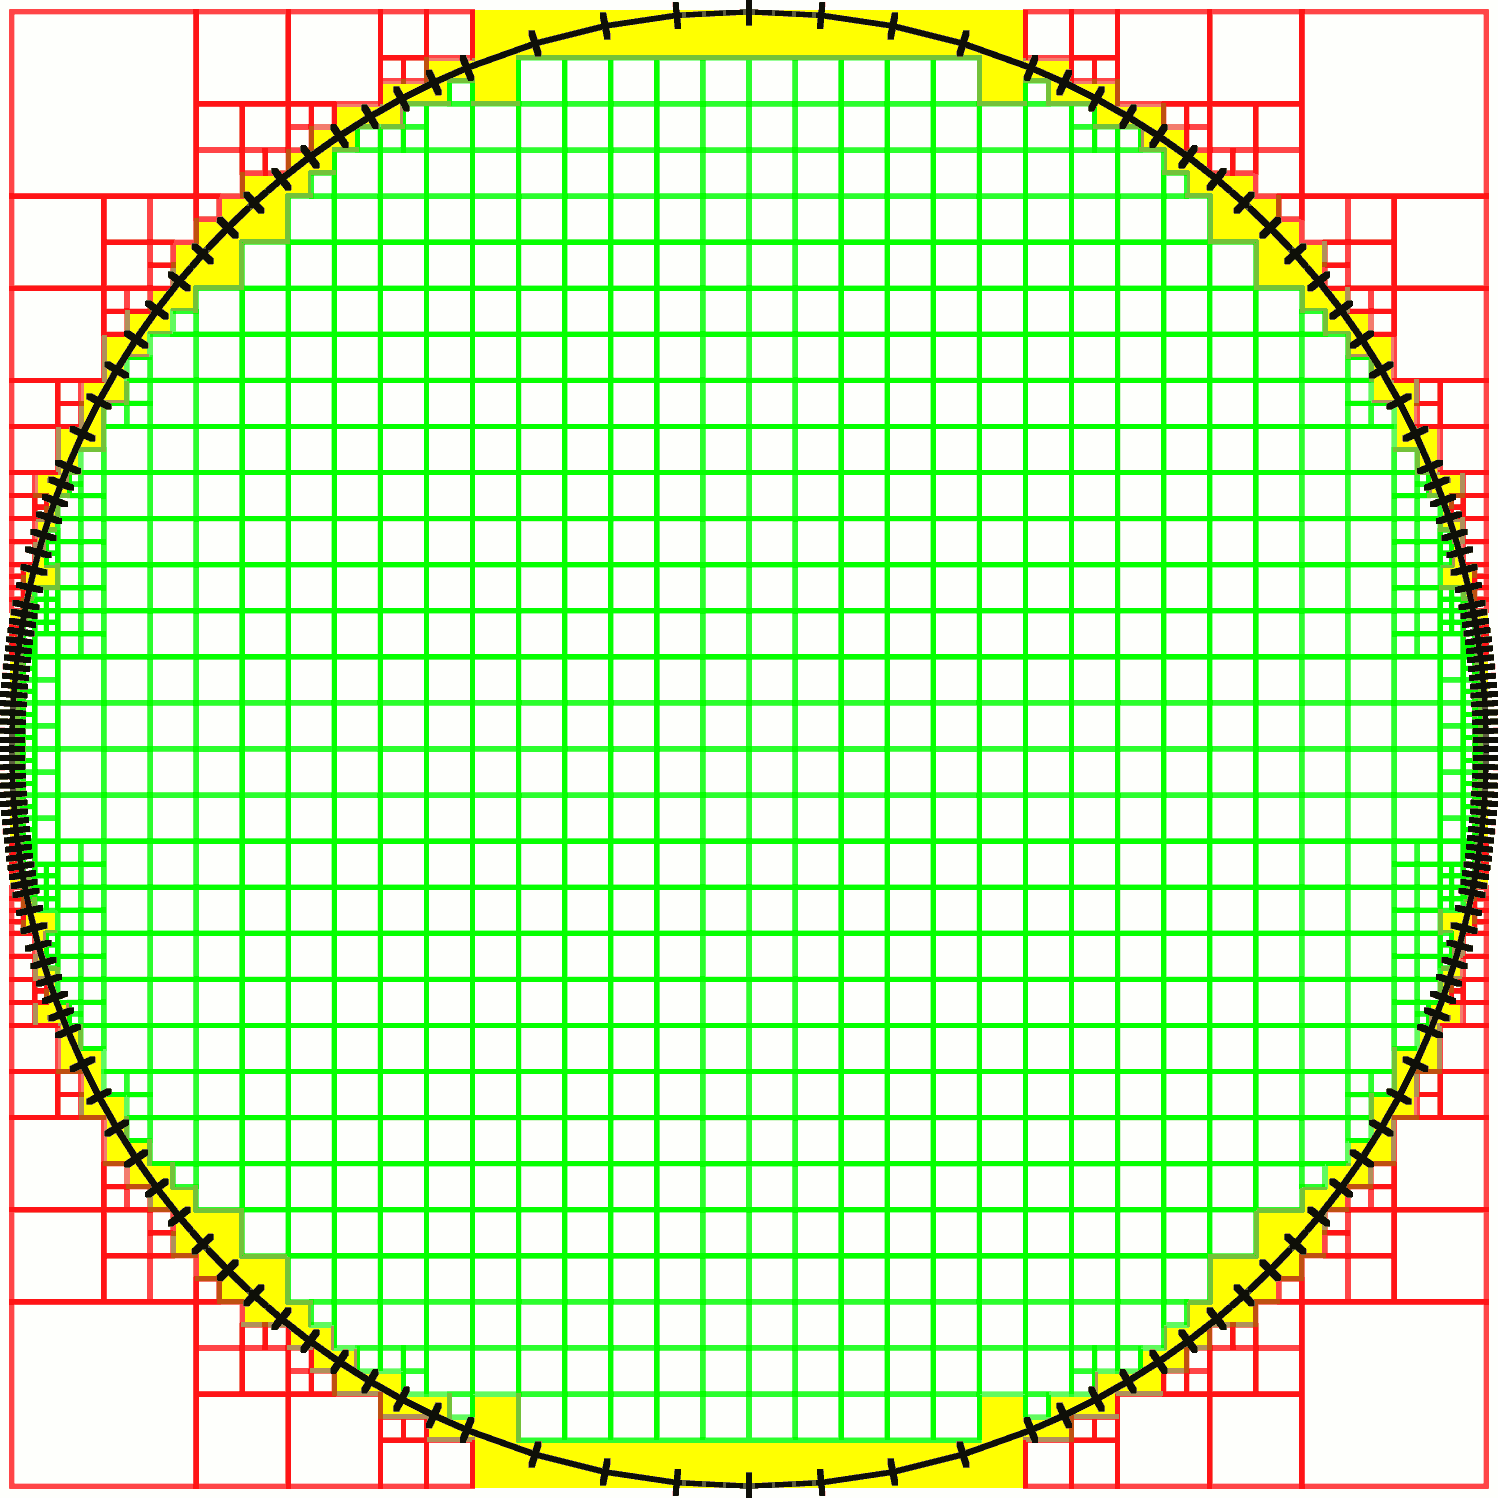
\includegraphics[width=0.4\textwidth]{fig/classificacao.png}
	\caption{\textit{Quadtree} de densidade com as células devidamente classificadas (células verdes - dentro do domínio, células vermelhas - fora do domínio, células amarelas - sobre a fronteira).}
	\label{fig:classificacao}
\end{figure}


\subsection{Cálculo da Carga}

A \textit{quadtree} de densidade é utilizada para fazer uma estimativa da carga neste trabalho. Com a sua construção é possível ter noção do tamanho dos elementos pertencentes ao domínio do objeto. Assim, uma ideia geral sobre a malha desejada é conhecida desde o início. A classificação das células folhas da \textit{quadtree} de densidade é utilizada para selecionar apenas as células que não estão fora do domínio de entrada, ou seja, as células que estão no interior do domínio e as que interceptam a borda (células verdes e amarelas na Figura \ref{fig:classificacao}). A quantidade dessas folhas não externas é considerada como a carga total para este domínio.

\section{Decomposição do Domínio}\label{sec:Decomposicao_dominio}

A técnica proposta neste trabalho tem apenas um pré-requisito quanto à estrutura de decomposição espacial para particionar o domínio dado como entrada. A estrutura de decomposição deve gerar regiões que sejam paralelas às células da \textit{quadtree} de densidade. Estruturas baseadas em árvore como \textit{quadtree}, \textit{octree}, BSP e \textit{Kd-tree} geram regiões que possibilitam a perfeita execução do algoritmo de geração dos subdomínios.

Vale lembrar que para um bom particionamento é preciso uma boa estimativa de carga e para se obter uma malha de boa qualidade depende-se de um bom particionamento do domínio. Para gerar exemplos e até mesmo para comparar os resultados dos diferentes tipos de estruturas de dados, esta seção descreve como é feita a criação de uma \textit{quadtree} e de uma BSP para decompor a entrada.

\subsection{Decomposição Utilizando BSP}

Uma excelente estrutura de particionamento é a BSP, aqui chamada de BSP de decomposição, tendo a sua criação guiada pela estrutura de estimativa de carga descrita anteriormente na Seção~\ref{sec:Estimativa_de_Carga}. A utilização desta estrutura foi baseada no trabalho de \cite{bib:RepMarkos13}, onde mais detalhes da construção e implementação podem ser encontrados nele. A BSP de decomposição pode ser construída de diversas formas, dependendo apenas do critério de subdivisão:


\begin{itemize}
	\item Subdivisão baseada na carga. Cada célula folha não pode ter uma carga maior que a carga média;
	\item Subdivisão baseada na diferença de carga total de cada as partições(Figura \ref{fig:bsp_decomposition_passos}); e 
	\item Subdivisão baseada no eixo mediano.
\end{itemize}


\begin{figure}[!ht]
	\centering
	\subfloat[Primeiro corte criado com pesos 5 para cada lado.]
	{\label{fig:bsp_decomposition_passos1}
		\begin{minipage}[c]{0.3\textwidth}{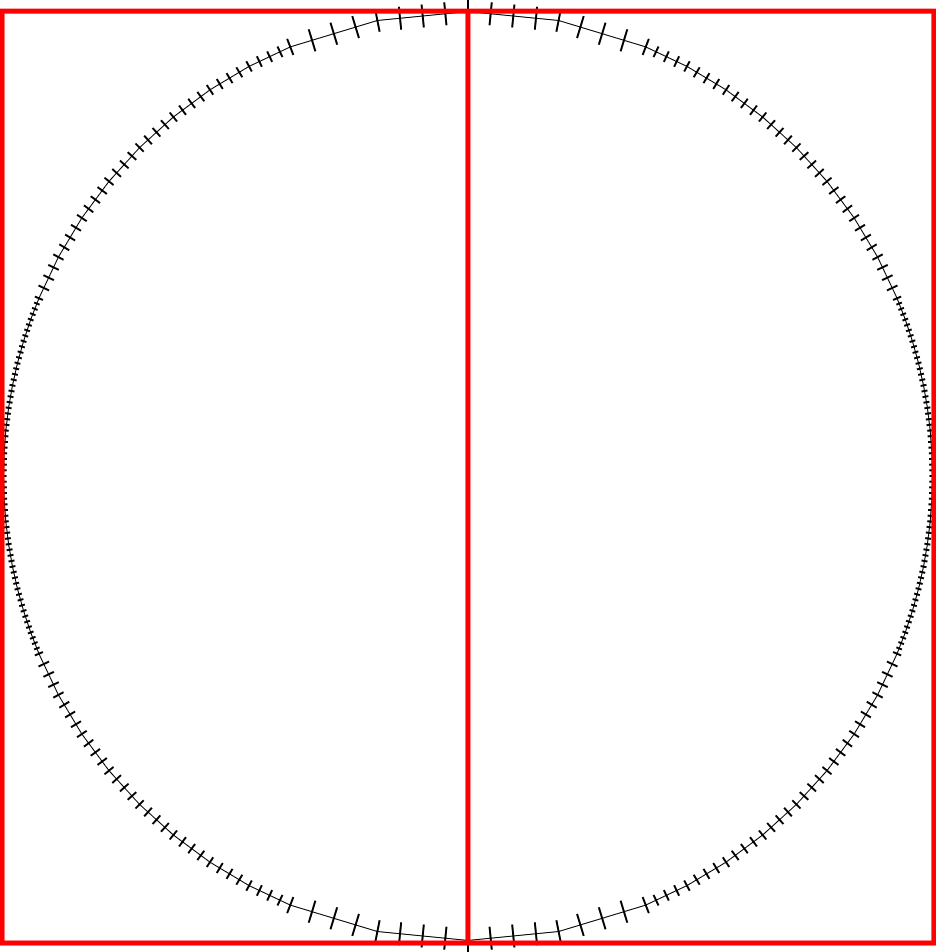
\includegraphics[width=\textwidth]{fig/bsp_passo1.png}}\end{minipage}
	}
	\qquad
	\subfloat[Segundo corte criado com pesos 2 e 3 para cada lado.]
	{\label{fig:bsp_decomposition_passos2}
		\begin{minipage}[c]{0.3\textwidth}{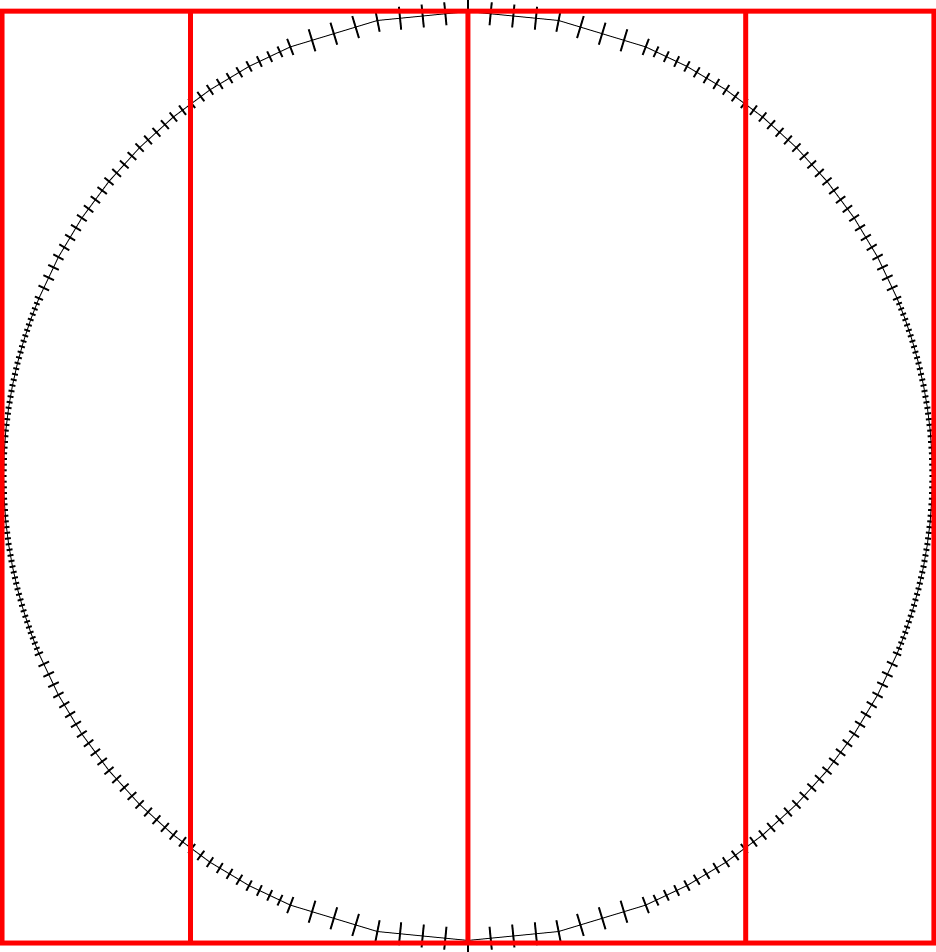
\includegraphics[width=\textwidth]{fig/bsp_passo2.png}}\end{minipage}
	}
	
	\subfloat[Terceiro corte criado gerando dois subdomínios.]
	{\label{fig:bsp_decomposition_passos3}
		\begin{minipage}[c]{0.3\textwidth}{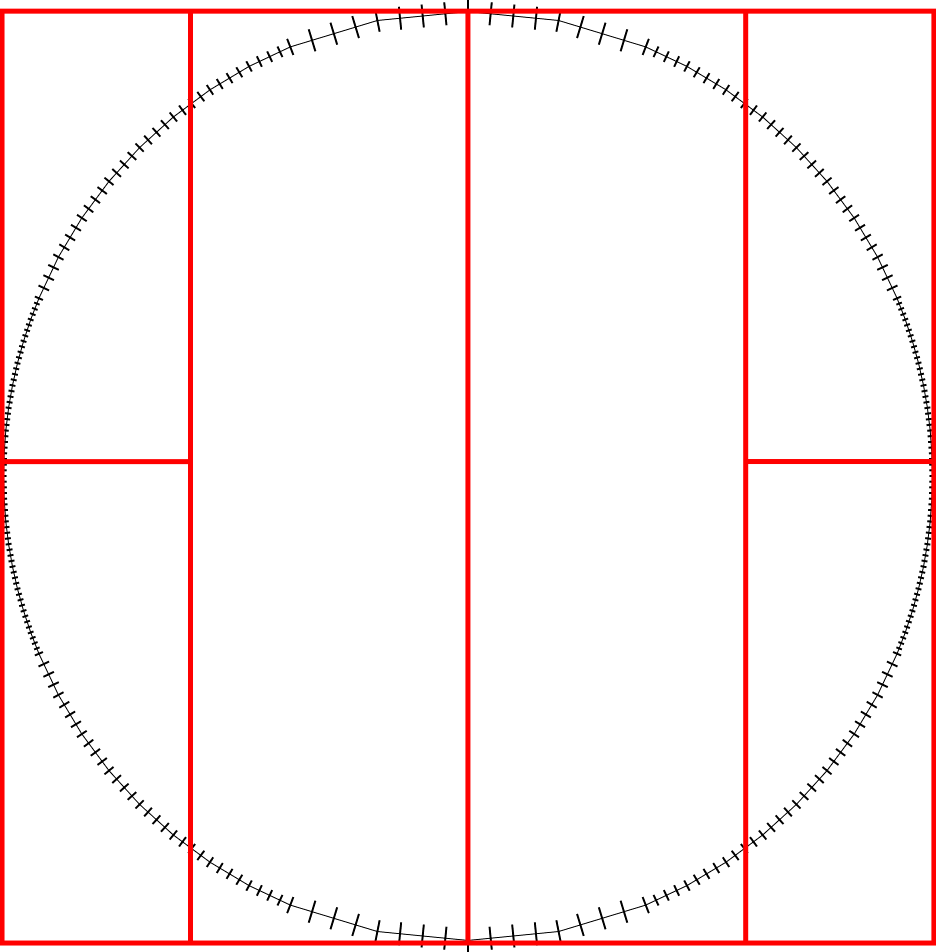
\includegraphics[width=\textwidth]{fig/bsp_passo3.png}}\end{minipage}
	}
	\qquad
	\subfloat[Último corte criado finalizando os 10 subdomínios.]
	{\label{fig:bsp_decomposition_passos4}
		\begin{minipage}[c]{0.3\textwidth}{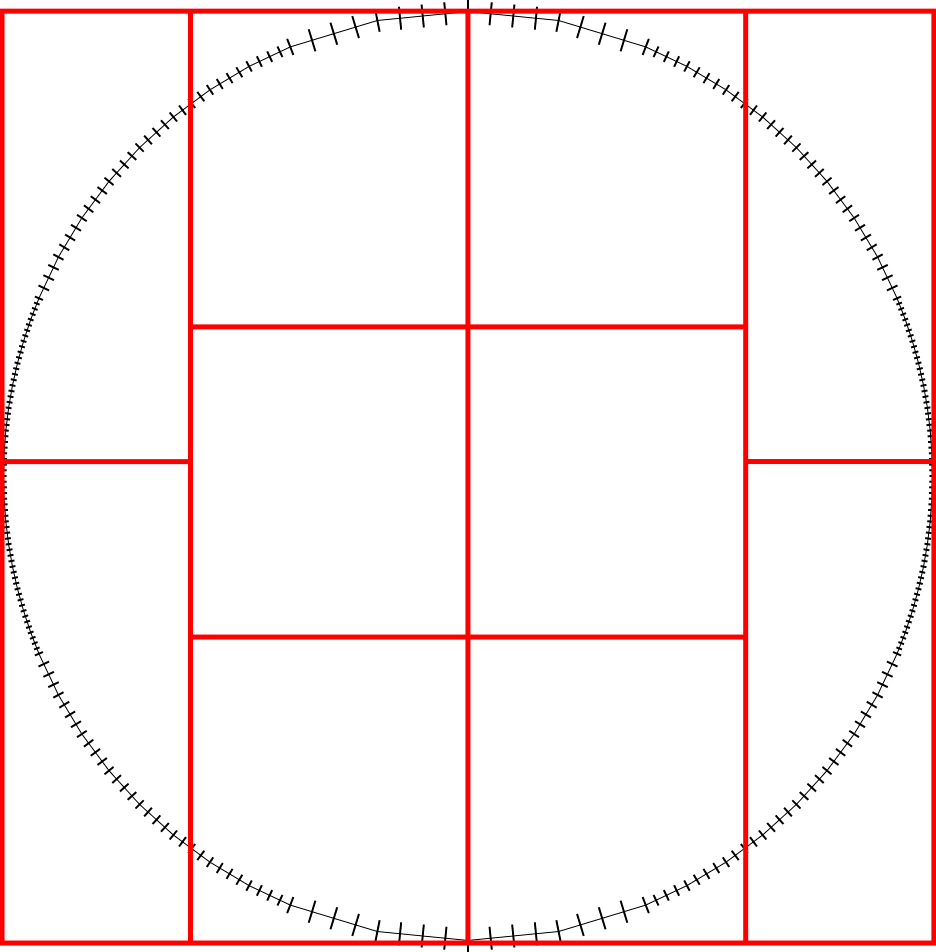
\includegraphics[width=\textwidth]{fig/bsp_passo4.png}}\end{minipage}
	}    
	\caption{Exemplo da criação de uma BSP bidimensional para 10 processadores baseada na diferença de carga.}
	\label{fig:bsp_decomposition_passos}
\end{figure}    


As principais vantagens da utilização de uma BSP são: a quantidade de subdivisões realizadas; e a liberdade que a BSP tem de subdividir o domínio em regiões de diferentes tamanhos. A possibilidade de gerar a quantidade de regiões que sejam necessárias com diferentes tamanhos torna o particionamento muito mais preciso. A Figura \ref{fig:bsp_decomposition_passos} mostra o passo a passo da criação de uma BSP de particionamento feita para dez processadores, ou seja, dez subdomínios foram criados.

Para gerar a BSP de decomposição a forma mais eficiente é a que faz a carga associada com cada uma das folhas ser menor que uma carga máxima pré-definida $L/P$, sendo $L$ a carga total da entrada e $P$ a quantidade de processadores disponíveis. Com a BSP, é possível obter $N=P$, sendo $N$ a quantidade de subdomínios criados, com uma carga de muito próxima a $L/P$ para cada $P$.

Inicia-se a BSP de decomposição com sua raiz definida como um quadrado, para o caso bidimensional, ou um cubo, para o caso tridimensional, envolvendo o domínio. A subdivisão é feita posicionando a partição no centro geométrico dessa célula, no eixo X. Se essa partição obtiver cargas iguais para os dois filhos, essa partição será a melhor para o eixo X. Caso contrário, seleciona-se a célula mais pesada e reposiciona-se o plano de partição para a metade dessa célula, no mesmo eixo. Esse procedimento é feito recursivamente até que as cargas dos dois subdomínios sejam iguais ou, quando atinge-se uma célula-folha da estrutura de estimativa, \textit{quadtree} para o caso bidimensional ou \textit{octree} para o caso tridimensional, ou seja, é impossível subdividir esta célula.

Esse procedimento é realizado em todos os eixos e ao final é selecionado o particionamento no eixo que melhor divide a carga nas duas novas células criadas. A Figura \ref{fig:passos_decomposicao_BSP} mostra o passo a passo da seleção da melhor subdivisão para o eixo X. Com essa subdivisão no eixo X, a diferença alcançada é de 4 (Figura \ref{fig:bsp_3}); porém, fazendo a decomposição no eixo Y a diferença seria de $0$. O particionamento selecionado vai ser o que obtiver a menor diferença, sendo assim, para o exemplo da Figura \ref{fig:bsp_3}, o particionamento selecionado seria o do Y.


\begin{figure}[ht]
	\centering
	\subfloat[\textit{Quadtree} de estimativa carga. Carga total: 52. Carga ideal de cada subdomínio: 26.]
	{\label{fig:bsp_0}
		\begin{minipage}[c]{0.3\textwidth}{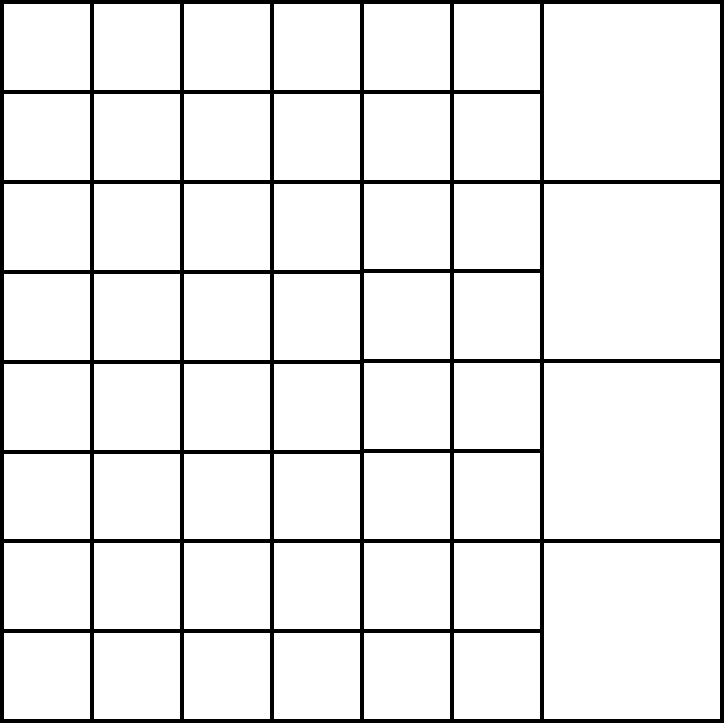
\includegraphics[width=\textwidth]{fig/bsp_0.png}}\end{minipage}
	}
	\qquad
	\subfloat[Posição inicial do plano de partição (em vermelho). Cargas dos subdomínios: 32 e 20. Diferença: 12.]
	{\label{fig:bsp_1}
		\begin{minipage}[c]{0.3\textwidth}{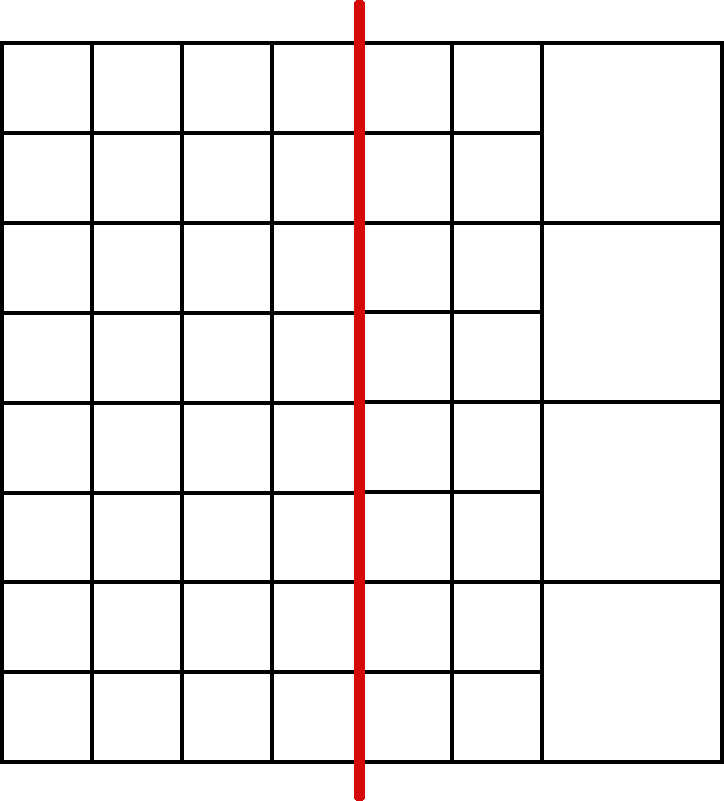
\includegraphics[width=\textwidth]{fig/bsp_1.png}}\end{minipage}
	}
	
	\subfloat[Deslocamento do plano de partição para o próximo nível da esquerda. Cargas dos subdomínios: 16 e 36. Diferença: 20.]
	{\label{fig:bsp_2}
		\begin{minipage}[c]{0.3\textwidth}{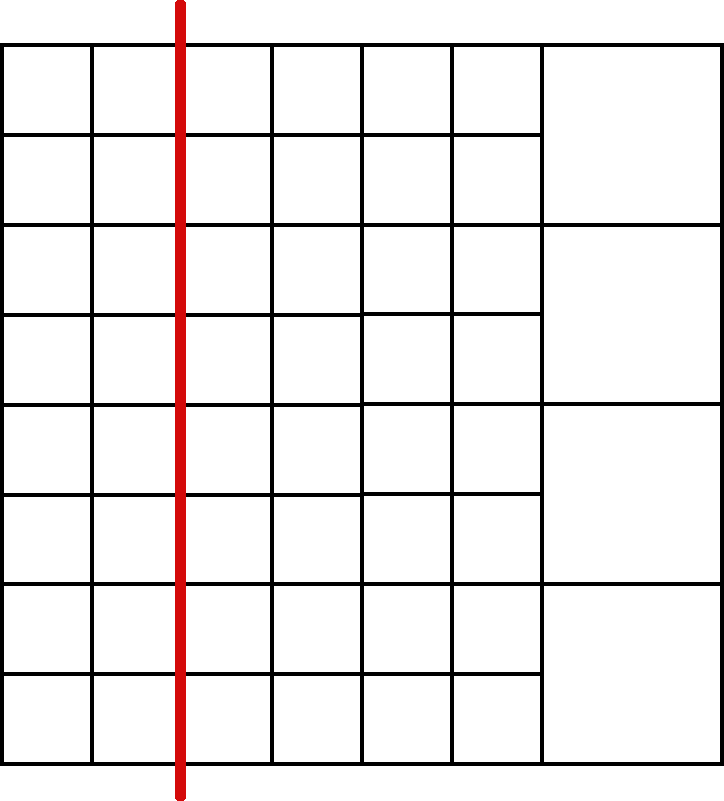
\includegraphics[width=\textwidth]{fig/bsp_2.png}}\end{minipage}
	}    
	\qquad
	\subfloat[Deslocamento do plano de partição para o próximo nível da direita. Cargas dos subdomínios: 24 e 28. Diferença: 4.]
	{\label{fig:bsp_3}
		\begin{minipage}[c]{0.3\textwidth}{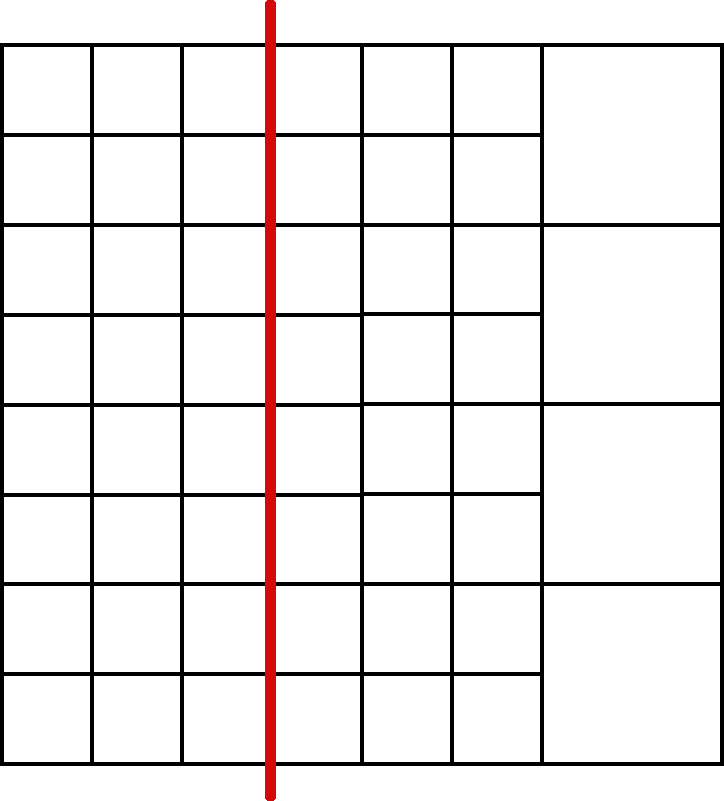
\includegraphics[width=\textwidth]{fig/bsp_3.png}}\end{minipage}
	}
	\caption{Passos de uma decomposição bidimensional de um domínio por BSP no eixo X para dois processadores, buscando a diferença mínima de carga total.}
	\label{fig:passos_decomposicao_BSP}
\end{figure}


Nos casos que o número de partições desejado seja ímpar, é aplicado um valor para indicar que a carga de uma região deve ser proporcional a $X$ vezes a de outra região. Com a aplicação desses pesos, é garantido que para qualquer quantidade de partições desejada, a BSP irá encontrar o melhor corte que dividirá a carga entre as partições. A Figura \ref{fig:circunferencia_cortejunto} mostra o processo de particionamento em uma circunferência para 3 regiões.

\begin{figure}[!ht]
	\centering
	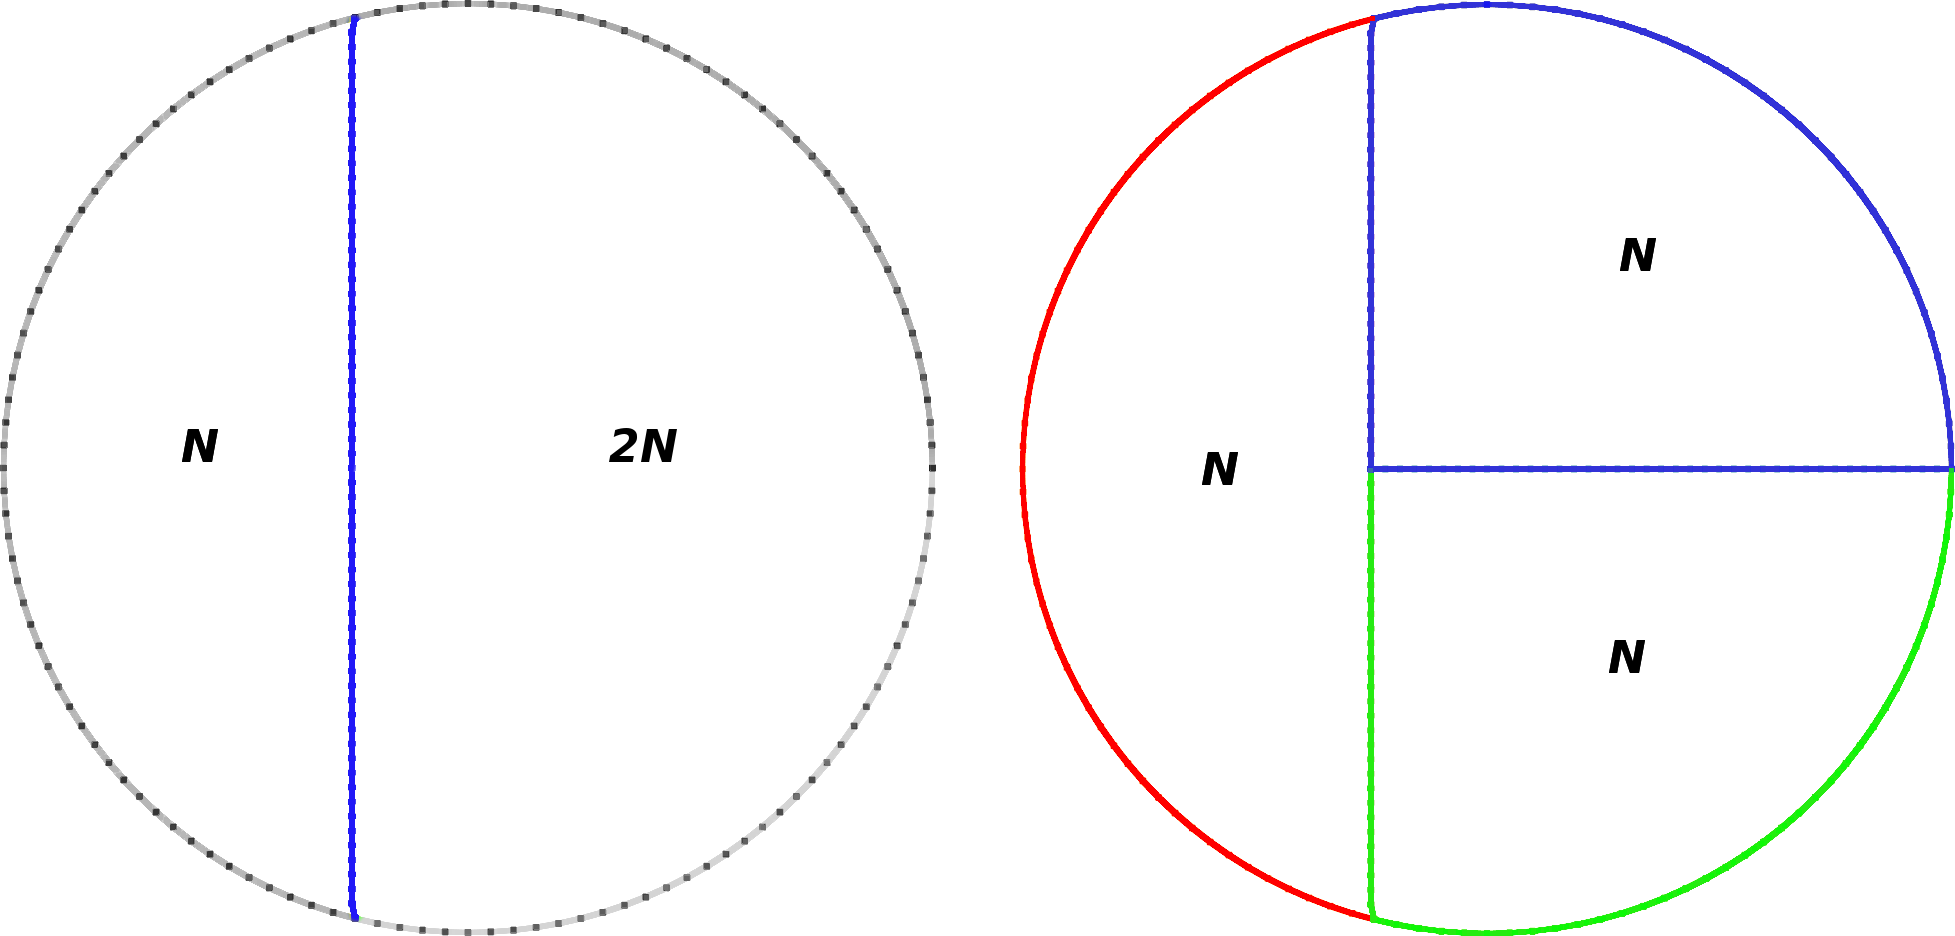
\includegraphics[width=0.7\textwidth]{fig/circunferencia_cortejunto.png}
	\caption{Proporção 2:1 é aplicada, fazendo um lado ter duas vezes mais carga que o outro (lado esquerdo). Resultado final é apresentado no lado esquerdo.}
	\label{fig:circunferencia_cortejunto}
\end{figure}

\section{Interfaces dos Subdomínios}

Na geração das interfaces dos subdomínios, é necessário ter a estrutura de estimativa de carga( uma \textit{quadtree} no caso bidimensional e uma \textit{octree} no caso tridimensional) e a estrutura de particionamento devidamente criadas(a BSP). Qualquer outra estrutura de decomposição espacial que gere regiões paralelas aos eixos pode ser utilizada nessa técnica de geração de subdomínios. 

Para construir a interface dos subdomínios é necessário possuir uma grade de suporte e os elementos do modelo de entrada em que a partição faz interseção. A grade de suporte irá guiar a a criação do elementos da interface, sendo ela responsável pelo tamanho e posicionamento dos mesmos. Os elementos do modelo que fazem interseção com a partição são necessários para fazer a junção da interface com o modelo, de tal modo que ao final não exista nenhum buraco na interface.

\subsection{Grade de Suporte}

Para cada corte da estrutura de particionamento é feito a interseção com as células folhas da estrutura de estimativa de carga (Figura \ref{fig:celulas_selecionadas2d_tree} para o caso bidimensional e Figura \ref{fig:celulas_selecionadas3d_tree} para o caso tridimensional). Como resultado dessa interseção, é obtido um conjunto de células da estrutura de estimativa de carga que cruzam ou apenas tangenciam a partição que se deseja criar. Essas células guiarão a criação das fronteiras dos seus respectivos subdomínios (células em azul nas Figuras \ref{fig:celulas_selecionadas2d_particoes} e \ref{fig:celulas_selecionadas3d_particoes}). A estrutura de estimativa de carga possui informações de tamanho, que são baseadas nas arestas da borda, essas informações ajudam na criação da malha de interface compatível com a discretização do domínio.

A Figura \ref{fig:celulas_selecionadas2d} mostra um exemplo do caso bidimensional da junção da \textit{quadtree} de estimativa de carga com uma BSP de particionamento e a sua interface gerada, já na Figura \ref{fig:celulas_selecionadas3d} mostra um exemplo para o caso tridimensional da junção da \textit{octree} de estimativa de carga com uma BSP de particionamento e a sua interface gerada.

\begin{figure}[!ht]
	\centering    
	\subfloat[\textit{Quadtree} de estimativa de carga junto com a BSP de particionamento.]
	{\label{fig:celulas_selecionadas2d_tree}
		\begin{minipage}[c]{0.45\textwidth}{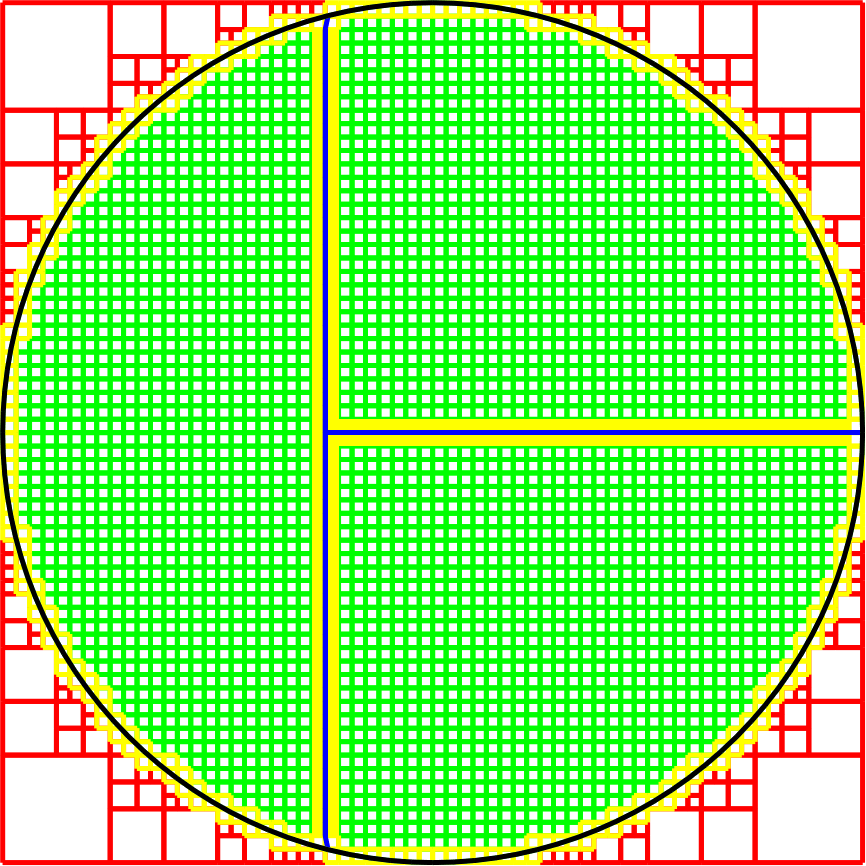
\includegraphics[width=\textwidth]{fig/circulo3_tree.png}}\end{minipage}
	}
	\qquad
	\subfloat[Interfaces do modelo gerada para três subdomínios.]
	{\label{fig:celulas_selecionadas2d_particoes}
		\begin{minipage}[c]{0.45\textwidth}{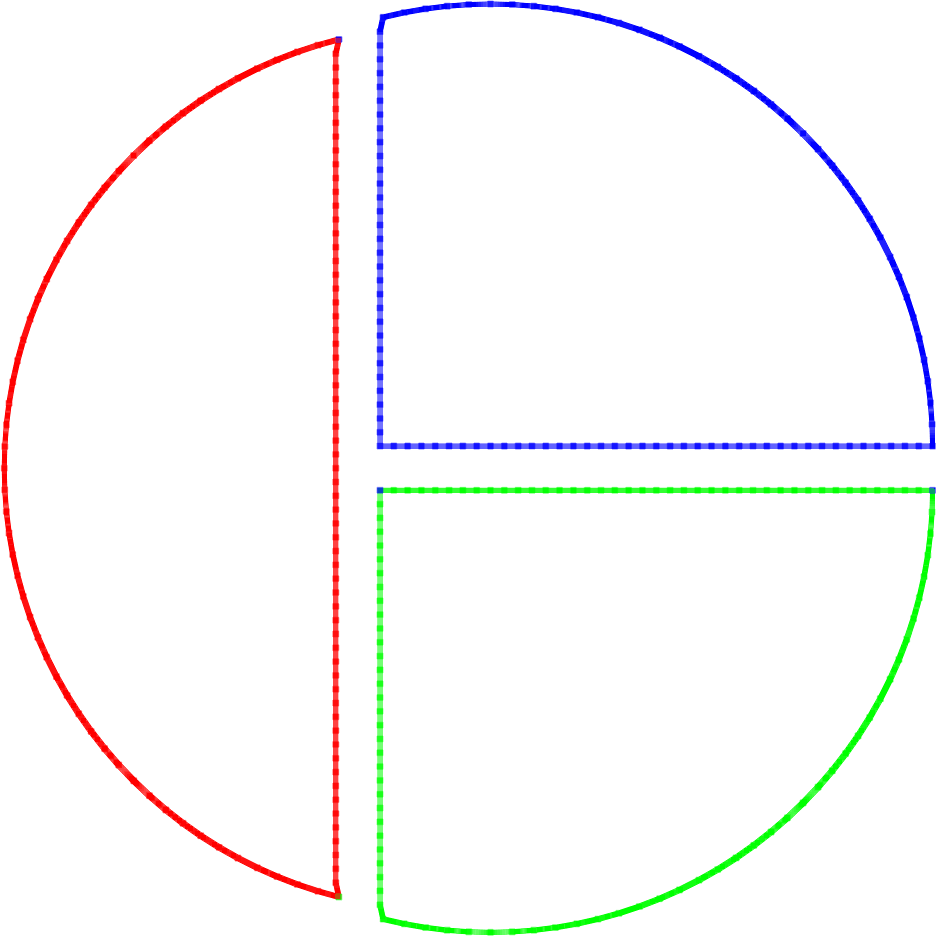
\includegraphics[width=\textwidth]{fig/circulo3.png}}\end{minipage}
	}
	\caption{Células da \textit{quadtree} de estimativa de carga em amarelo escuro serão utilizadas para guiar a criação da borda dos novos subdomínios.}
	\label{fig:celulas_selecionadas2d}
\end{figure}


\begin{figure}[!ht]
	\centering    
	\subfloat[\textit{Octree} de estimativa de carga junto com a BSP de particionamento.]
	{\label{fig:celulas_selecionadas3d_tree}
		\begin{minipage}[c]{0.45\textwidth}{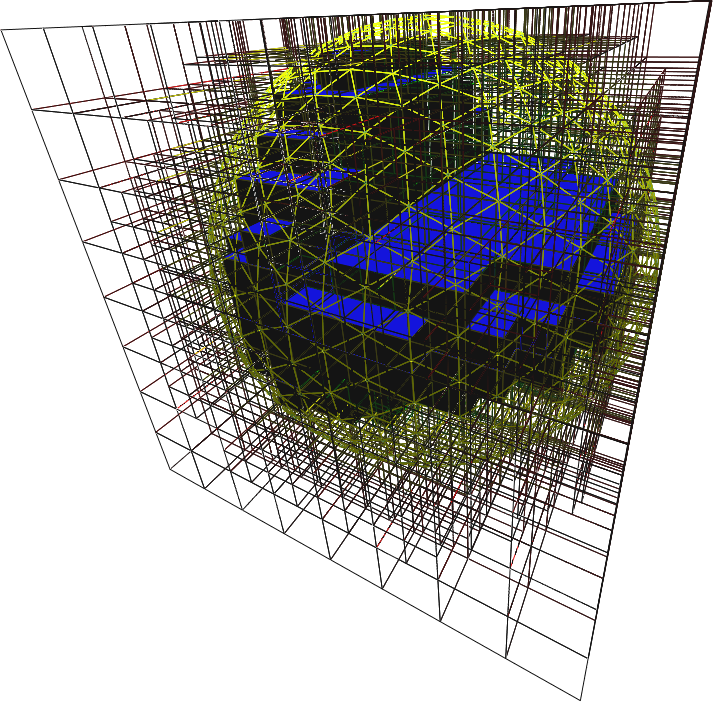
\includegraphics[width=\textwidth]{fig/esfera3_tree.png}}\end{minipage}
	}
	\qquad
	\subfloat[Interfaces do modelo gerada para três subdomínios.]
	{\label{fig:celulas_selecionadas3d_particoes}
		\begin{minipage}[c]{0.45\textwidth}{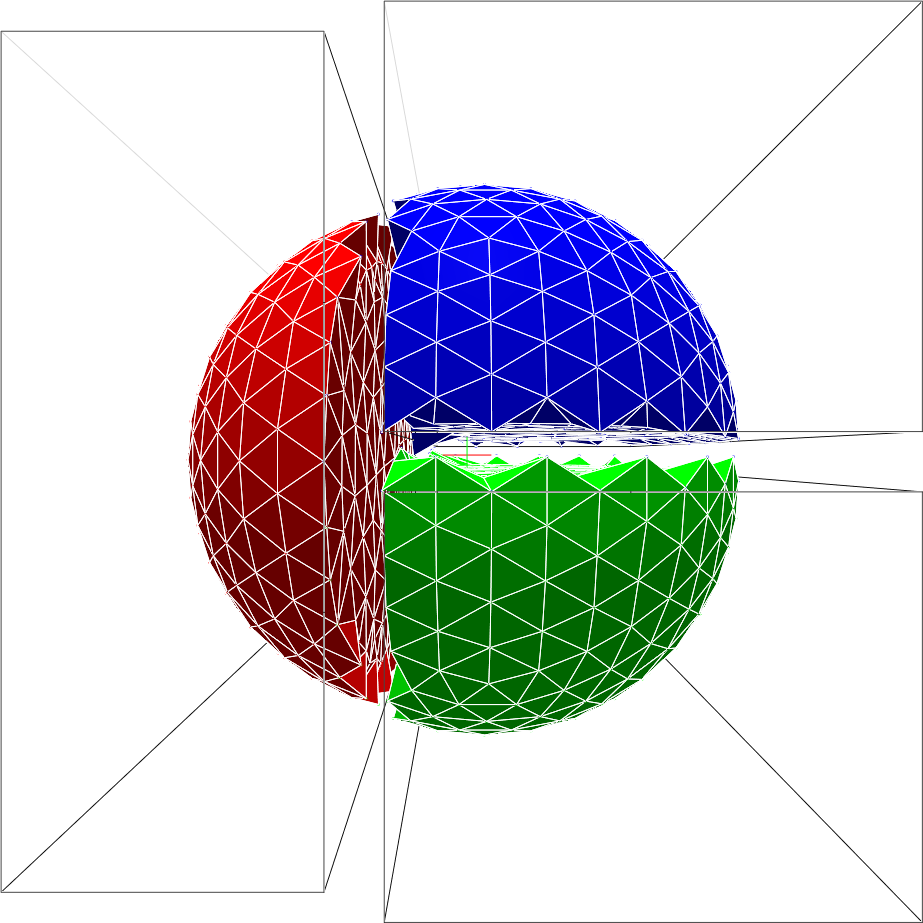
\includegraphics[width=\textwidth]{fig/esfera3.png}}\end{minipage}
	}
	\caption{Células da \textit{octree} de estimativa de carga em azul serão utilizadas para guiar a criação da borda dos novos subdomínios.}
	\label{fig:celulas_selecionadas3d}
\end{figure}


Células que estão totalmente fora da fronteira do domínio, ou seja, que não estão dentro e nem sobre a fronteira do domínio, mas que também fazem interseção com a estrutura de particionamento, não devem fazer parte desse conjunto. Como essas células estão totalmente fora do domínio, não haverá criação de interfaces nessas regiões; logo, elas devem ser retiradas desse conjunto.

Agora com o conjunto de células internas que interceptam a partição totalmente montado, é feita a construção da grade de suporte, tendo como base as menores células deste conjunto. Na Figura \ref{fig:criacao_1} as célula em azul escuro são externas ao subdomínio e as azul claro são internas. Após as menores células serem selecionadas o resultado é mostrado na Figura \ref{fig:criacao_2}.


     \begin{figure}[!ht]
     	\centering
     	\subfloat[Exemplo onde a \textit{quadtree} de densidade possui células de tamanhos diferentes.]
     	{\label{fig:criacao_1}
     		\begin{minipage}[c]{0.3\textwidth}{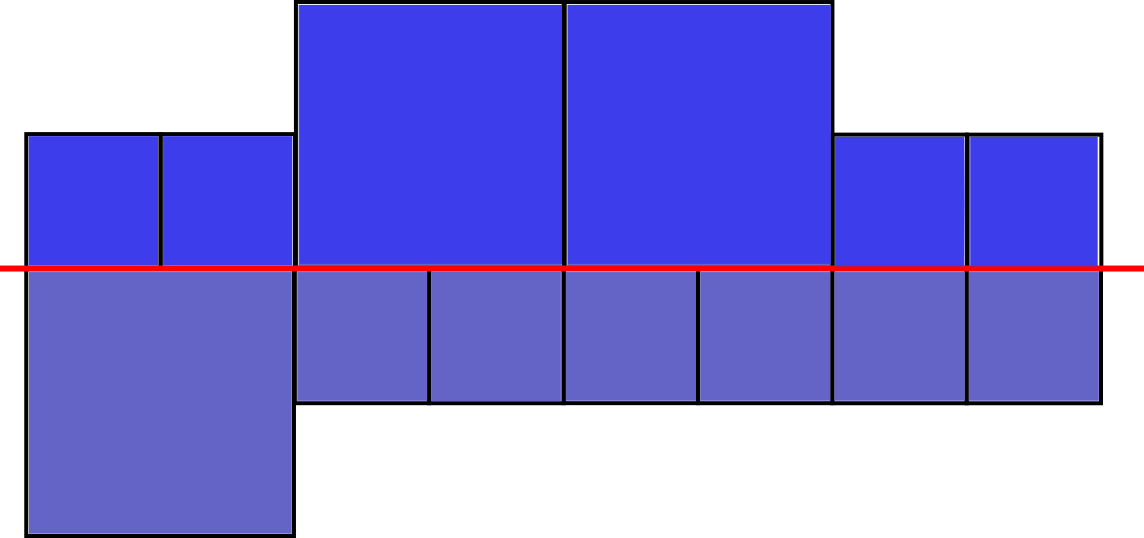
\includegraphics[width=\textwidth]{fig/criacao_1.png}}\end{minipage}
     	}
     	\qquad
     	\subfloat[Células em azul foram as selecionadas para geração da grade de suporte.]
     	{\label{fig:criacao_2}
     		\begin{minipage}[c]{0.3\textwidth}{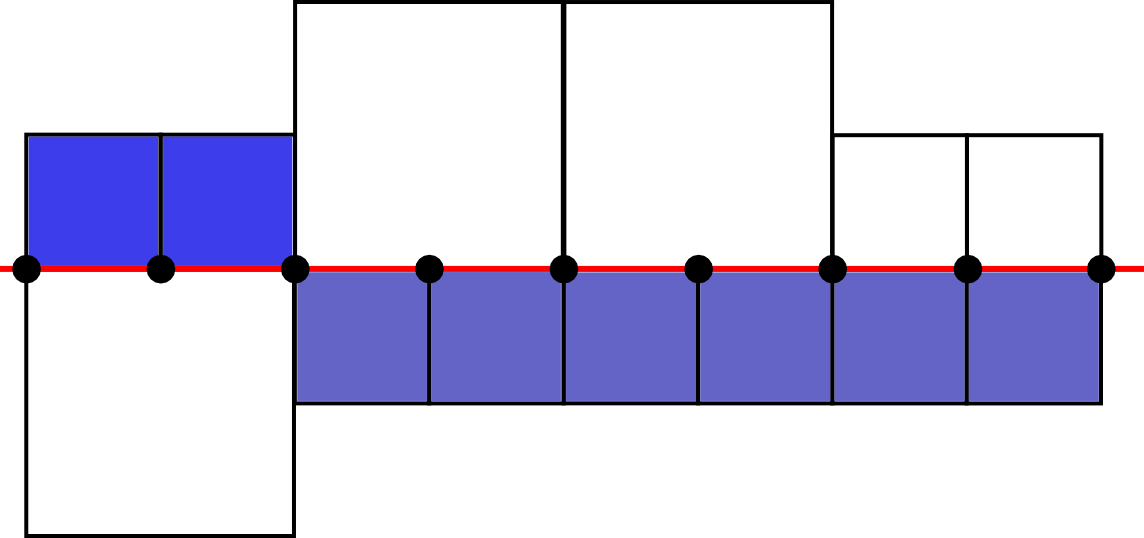
\includegraphics[width=\textwidth]{fig/criacao_2.png}}\end{minipage}
     	}    
     	\caption{Processo de criação da grade de suporte para o caso bidimensional.}
     	\label{fig:criacao_arestas}
     \end{figure}   

No caso bidimensional a grade de suporte é apenas um conjunto de pontos, já no caso tridimensional é feita uma triangulação bidimensional usando padrões nos vértices previamente selecionados. A Figura \ref{fig:grades_modelos} mostra a grade de suporte que foi gerada para um modelo bidimensional e um tridimensional.


     \begin{figure}[!ht]
     	\centering
     	\subfloat[Grade de suporte resultante do corte que passa entre a partição vermelha e a junção da partição azul com a verde da Figura \ref{fig:celulas_selecionadas2d_particoes}.]
     	{\label{fig:grades_modelos2d}
     		\begin{minipage}[c]{0.4\textwidth}{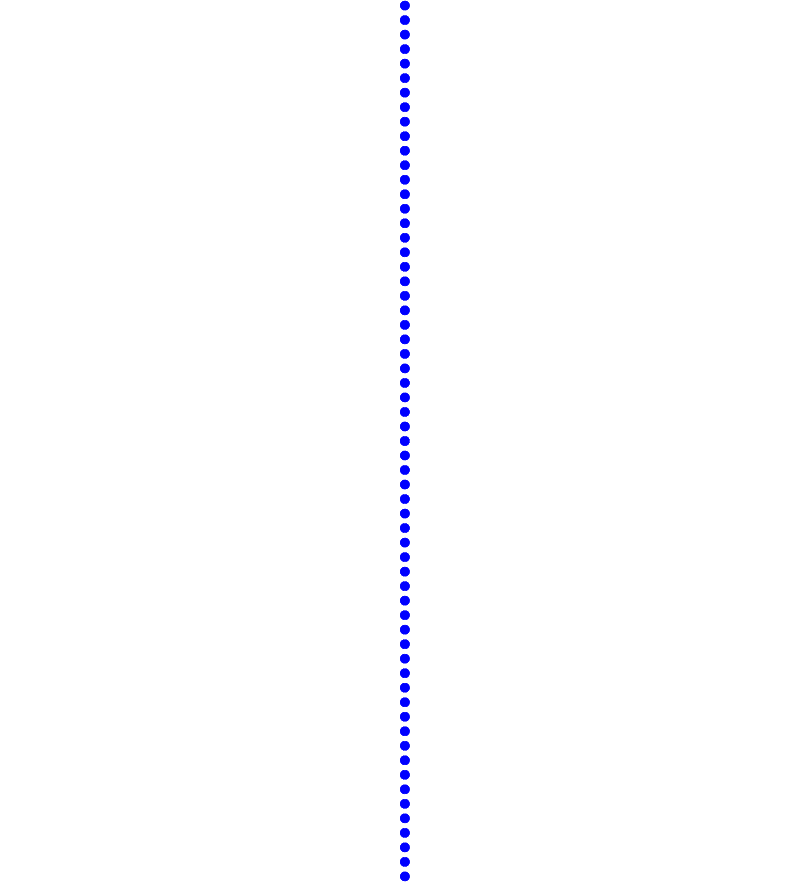
\includegraphics[width=\textwidth]{fig/circulo3_grade.png}}\end{minipage}
     	}
     	\qquad
     	\subfloat[Grade de suporte resultante do corte que passa entre a partição vermelha e a junção da partição azul com a verde da Figura \ref{fig:celulas_selecionadas3d_particoes}.]
     	{\label{fig:grades_modelos3d}
     		\begin{minipage}[c]{0.4\textwidth}{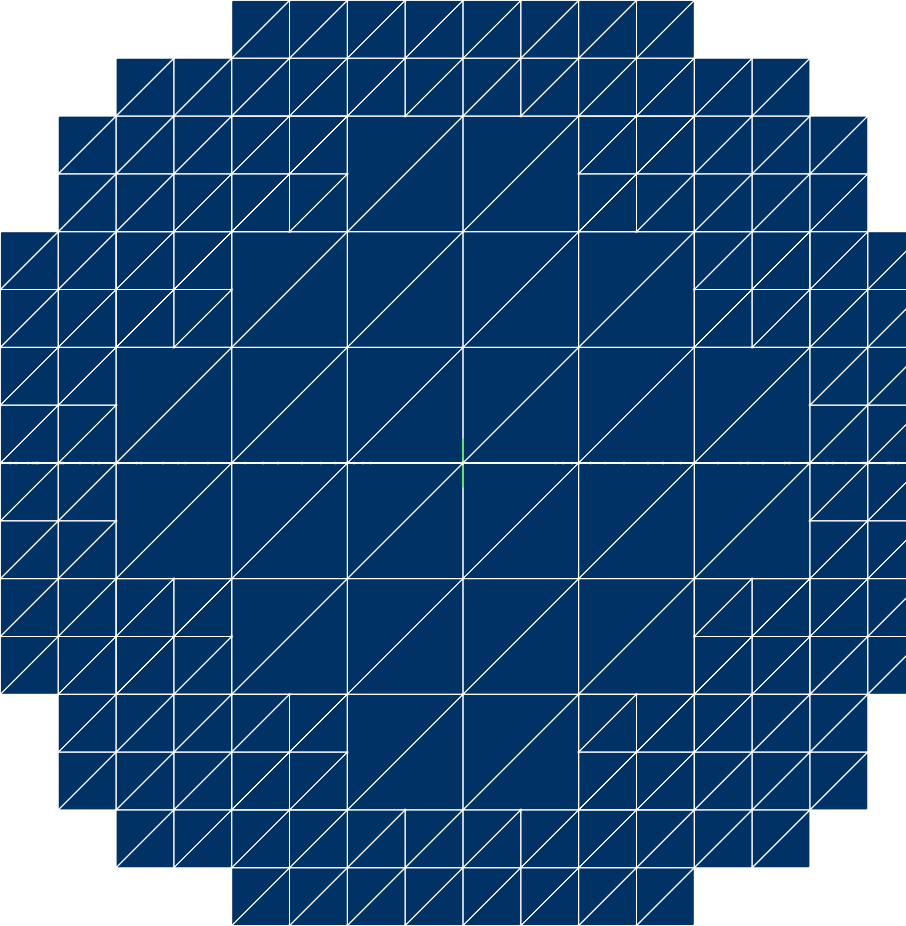
\includegraphics[width=\textwidth]{fig/esfera3_grade.png}}\end{minipage}
     	}    
     	\caption{Grades de suporte para o caso bidimensional e tridimensional.}
     	\label{fig:grades_modelos}
     \end{figure}
     
        
\subsection{Elementos de Interseção}

Algumas partições estarão sobre a fronteira do domínio e alguns de seus elementos terão que se conectar à esta fronteira. O caso bidimensional é simples quando comparado ao caso tridimensional.

No caso bidimensional é feita a interseção das arestas do modelo com o corte posicionado pela BSP de particionamento. O conjunto de arestas resultante serão as candidatas a fazerem parte da malha de interface. A Figura \ref{fig:circulo_arestas} ilustra o resultado obtido para o caso bidimensional.


\begin{figure}[!ht]
	\centering
	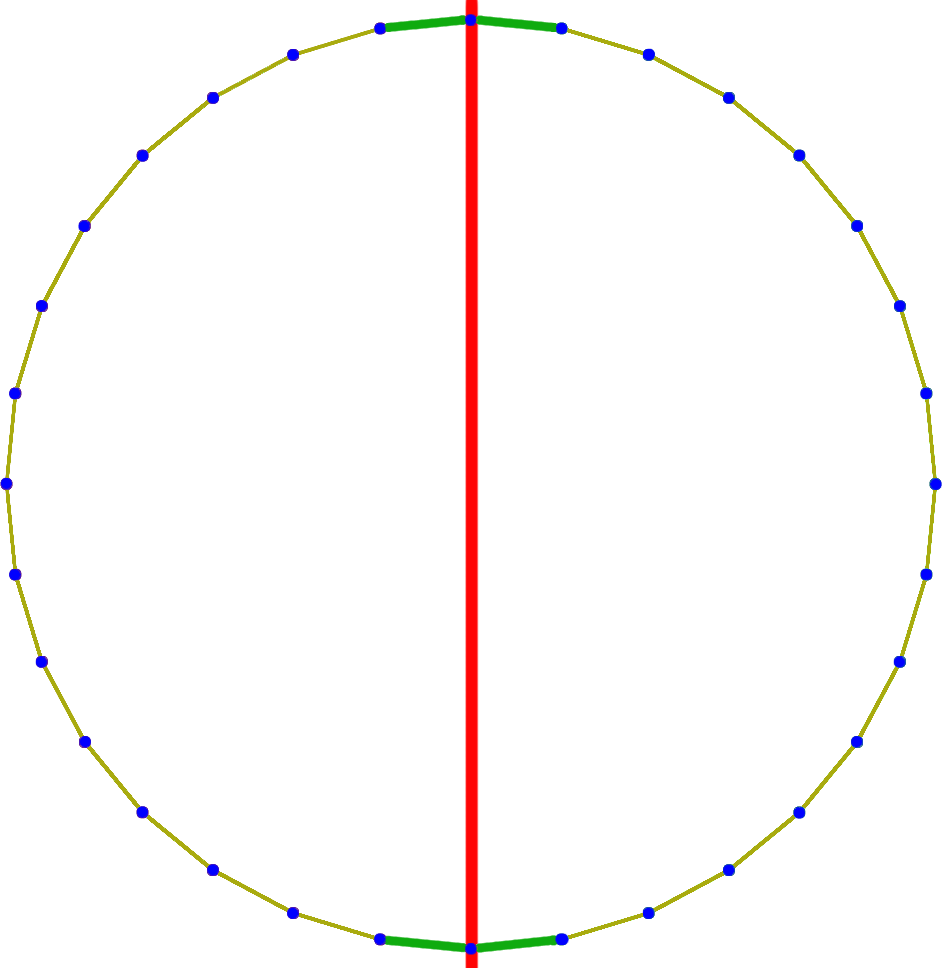
\includegraphics[width=0.35\textwidth]{fig/circulo2_arestas.png}
	\caption{Arestas em verde serão selecionadas ao fazer a interseção do corte feito pela BSP com o modelo.}
	\label{fig:circulo_arestas}
\end{figure}


Já no caso tridimensional a interseção das faces do modelo com o corte posicionado pela BSP de particionamento irá resultar em um conjunto de faces. A Figura \ref{fig:espera_faces} ilustra o resultado obtido para o caso tridimensional. Baseado nestas faces, é necessário encontrar o melhor ciclo de arestas possível.


\begin{figure}[!ht]
   	\centering
   	\subfloat[Interseção do plano de partição da BSP com o modelo. As faces em azul fazem insterseção com o plano.]
   	{\label{fig:espera_modelos_faces}
   		\begin{minipage}[c]{0.4\textwidth}{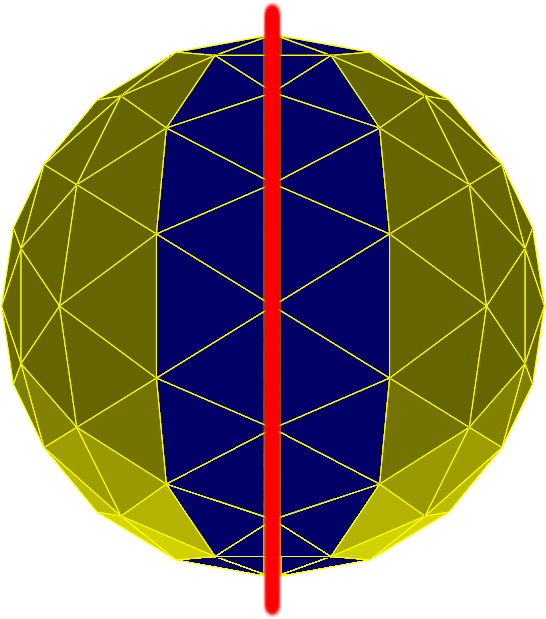
\includegraphics[width=\textwidth]{fig/esfera_simples_particao.png}}\end{minipage}
   	}
   	\qquad
   	\subfloat[Visão lateral das faces que fazem insterseção com o plano de partição da BSP.]
   	{\label{fig:espera_faces_selecionadas}
   		\begin{minipage}[c]{0.4\textwidth}{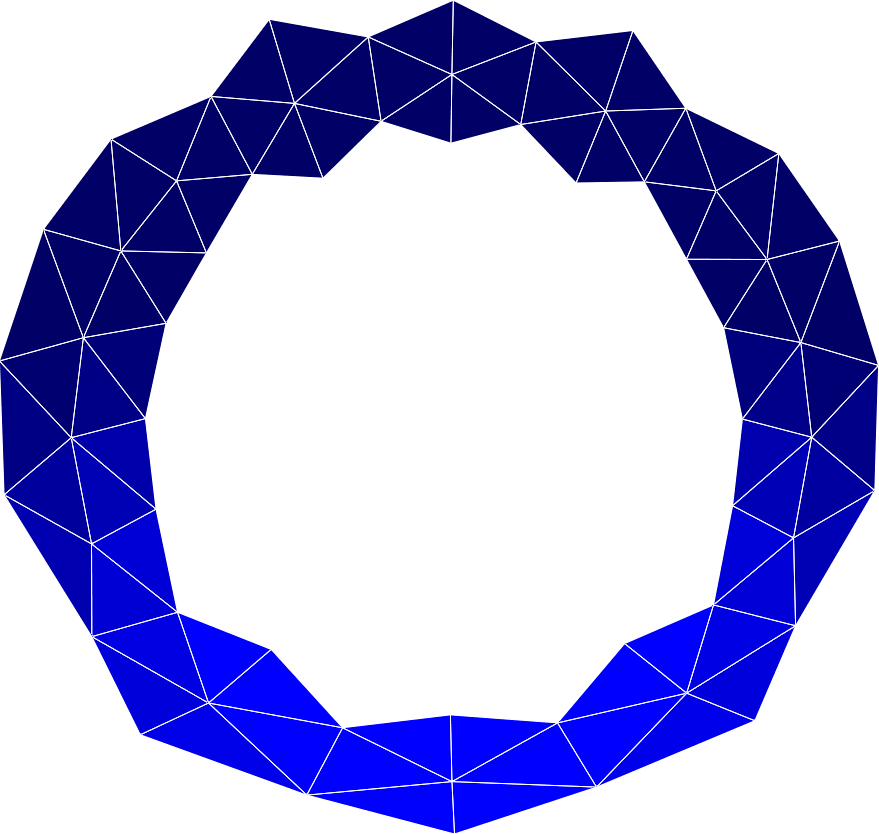
\includegraphics[width=\textwidth]{fig/esfera_simples_anel_faces.png}}\end{minipage}
   	}    
   	\caption{Passos para encontrar o conjunto do faces que fazem interseção com o plano de partição feito pela BSP.}
   	\label{fig:espera_faces}
\end{figure}


O critério de seleção inicial das arestas é obter todas as arestas que interceptam o plano de partição, eliminando aquelas fique ficarem soltas ou que formem pequeno ciclos. Ao final é obtido um ciclo, não necessariamente ele será o melhor, por isso é necessário realizar mais um passo de melhoria deste ciclo de arestas. A Figura \ref{fig:melhoria_arestas_faces_ruim1} e \ref{fig:melhoria_arestas_faces_ruim2} ilustram em vermelho o ciclo inicial de arestas encontrado, tendo como base as faces do modelo que interceptaram o plano de partição da BSP.

\begin{figure}[ht]
	\centering
	\subfloat[Modelo 01: Arestas selecionadas inicialmente.]
	{\label{fig:melhoria_arestas_faces_ruim1}
		\begin{minipage}[c]{0.3\textwidth}{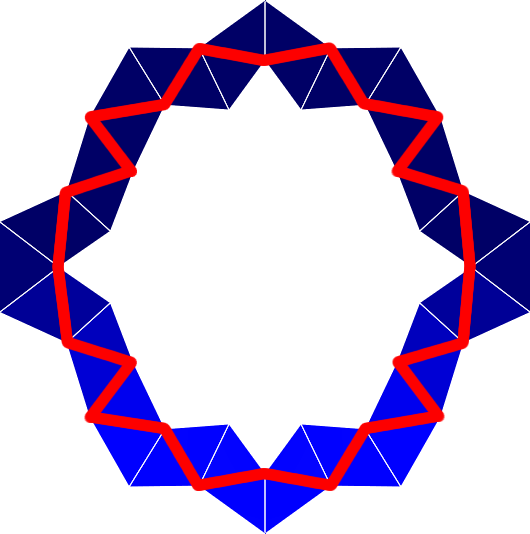
\includegraphics[width=\textwidth]{fig/exemplo_arestas_ruim1.png}}\end{minipage}
	}
	\qquad
	\subfloat[Modelo 01: Melhoria realizada na arestas previamente selecionadas.]
	{\label{fig:melhoria_arestas_faces_bom1}
		\begin{minipage}[c]{0.3\textwidth}{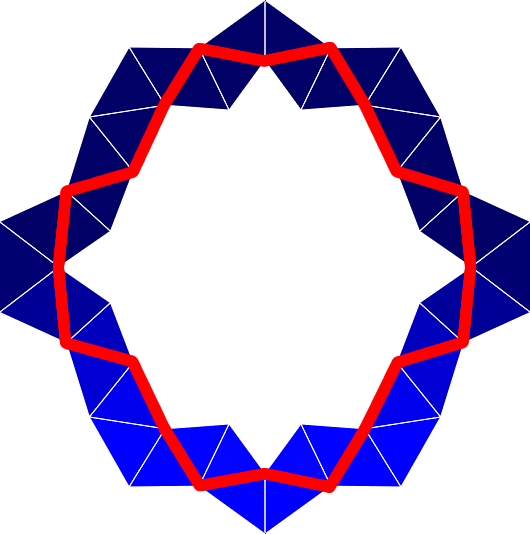
\includegraphics[width=\textwidth]{fig/exemplo_arestas_bom1.png}}\end{minipage}
	}
	
	\subfloat[Modelo 02: Arestas selecionadas inicialmente.]
	{\label{fig:melhoria_arestas_faces_ruim2}
		\begin{minipage}[c]{0.3\textwidth}{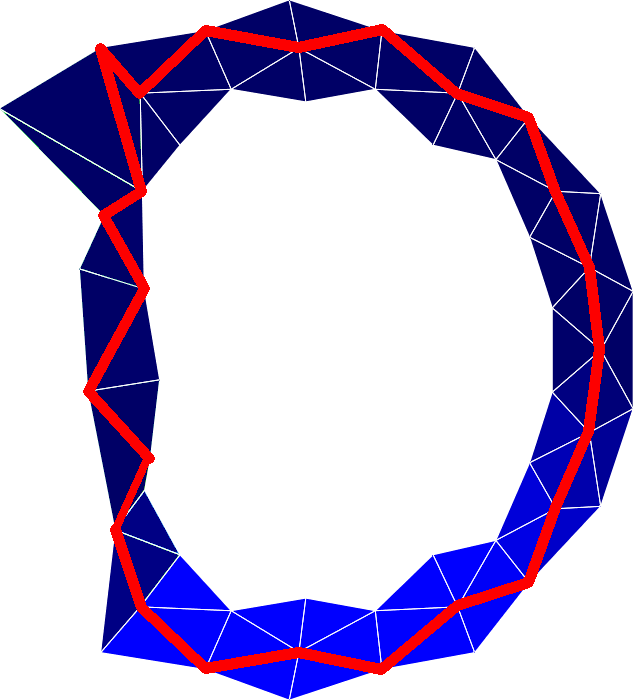
\includegraphics[width=\textwidth]{fig/exemplo_arestas_ruim2.png}}\end{minipage}
	}    
	\qquad
	\subfloat[Modelo 02: Melhoria realizada na arestas previamente selecionadas.]
	{\label{fig:melhoria_arestas_faces_bom2}
		\begin{minipage}[c]{0.3\textwidth}{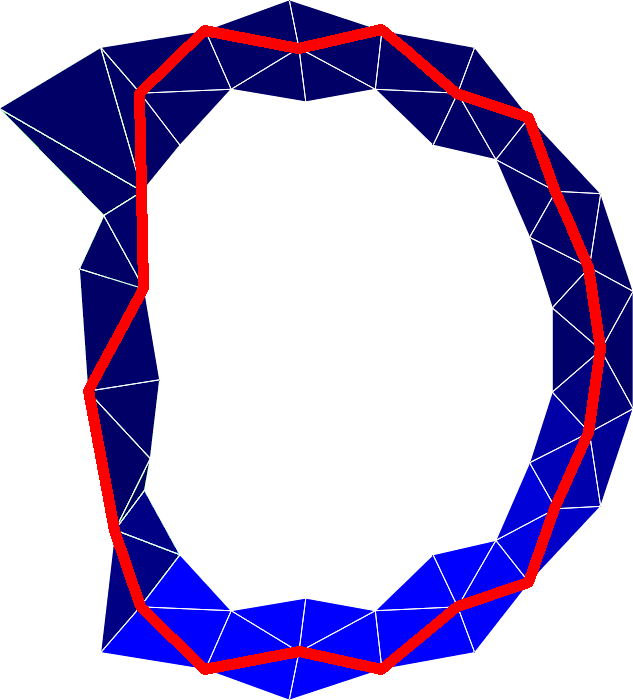
\includegraphics[width=\textwidth]{fig/exemplo_arestas_bom2.png}}\end{minipage}
	}
	\caption{Seleção do ciclo de arestas (em vermelho) com e sem melhoria.}
	\label{fig:melhoria_arestas_faces}
\end{figure}


A melhoria do ciclo de arestas é feito visando melhorar o angulo entre as arestas, consequentemente melhorará a malha de interface que será gerada. Para cada par de arestas vizinhas é feito uma verificação se existe uma face que contém estas duas arestas, se existir e o angulo entre as arestas melhorar, estas duas arestas serão removidas e será adicionada a outa aresta da face encontrada. Um exemplo pode ser visto da Figura \ref{fig:melhoria_arestas_faces} onde é possível ver as mudanças que ocorreram quando a melhoria foi realizada.

\subsection{Geração da Interface Bidimensional}

No caso bidimensional as arestas da interface são criadas seguindo a grade de pontos encontrada anteriormente. É necessário realizar a junção dessas arestas com o modelo, para isto é feito uma busca nos vértices que fazem interseção com a partição. O vértice que formar o maior angulo com a interface será o candidato para realizar a junção da interface com o modelo. Ao final desse processo cada partição terá sua fronteira construída e estará pronta para geração da malha.


\subsubsection{Teste de Proximidade}
\label{sec:Teste_proximidade}

Um dos problemas de se utilizar estruturas que geram regiões paralelas aos eixos para particionar domínios é a possibilidade das partições estarem posicionadas em regiões onde os elementos a serem gerados sejam de má qualidade ou até mesmo em posições em que não é possível gerar elementos (a Figura \ref{fig:teste_prox1} mostra um caso da partição estar muito próxima da fronteira). 


\begin{figure}[ht]
	\centering
	\subfloat[Caso em que o tratamento de proximidade é realizado.]
	{\label{fig:teste_prox1}
		\begin{minipage}[c]{0.35\textwidth}{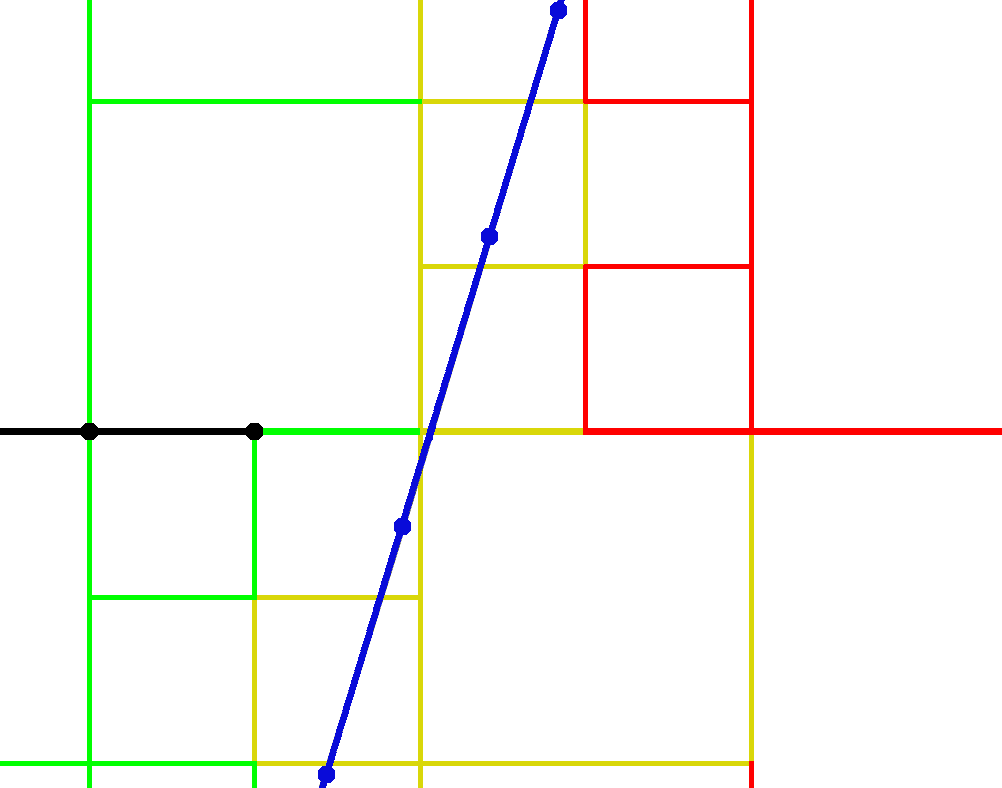
\includegraphics[width=\textwidth]{fig/teste_prox1.png}}\end{minipage}
	}
	\qquad
	\subfloat[Busca pelo vértice da fronteira que forma o maior angulo entre os candidatos.]
	{\label{fig:teste_prox2}
		\begin{minipage}[c]{0.35\textwidth}{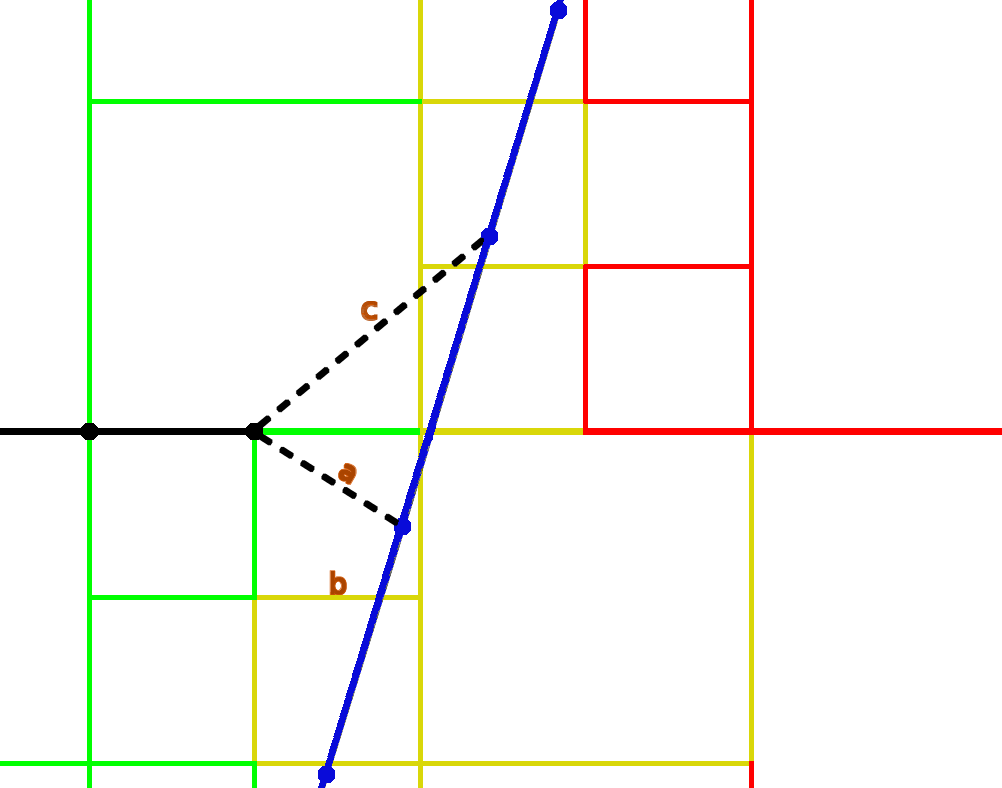
\includegraphics[width=\textwidth]{fig/teste_prox2.png}}\end{minipage}
	}
	
	\subfloat[Aresta criada pelo teste de proximidade.]
	{\label{fig:teste_prox_fim}
		\begin{minipage}[c]{0.35\textwidth}{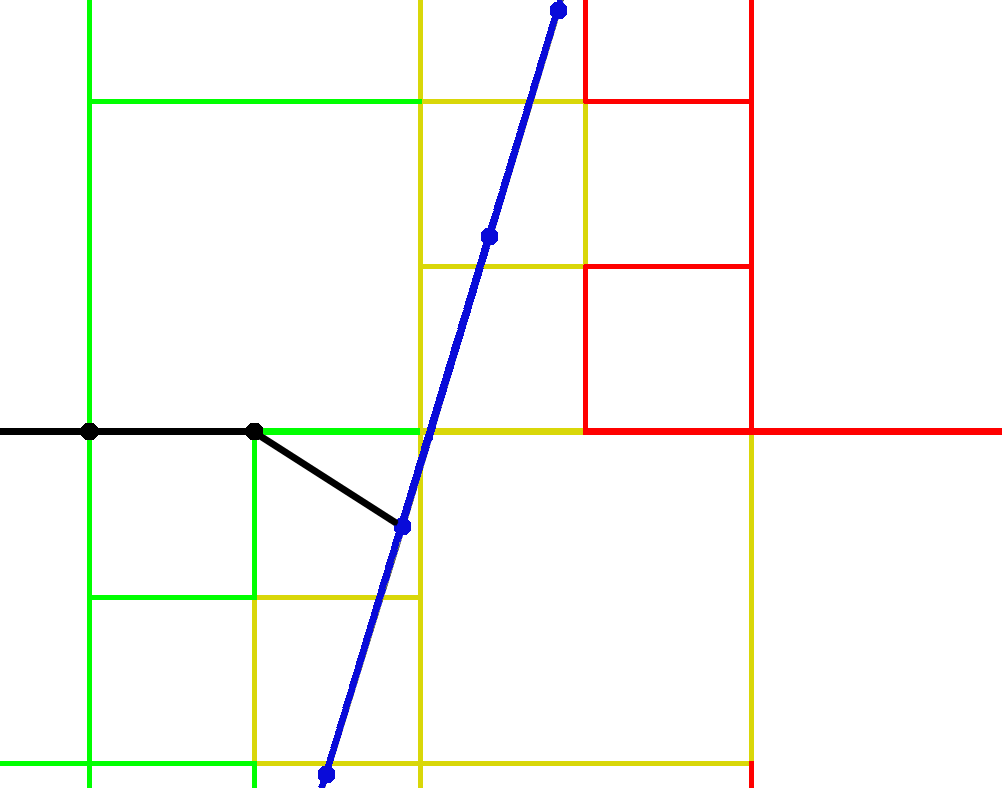
\includegraphics[width=\textwidth]{fig/teste_prox_fim.png}}\end{minipage}
	}    
	\qquad
	\subfloat[Aresta que seria criada caso o teste de proximidade não fosse realizado.]
	{\label{fig:teste_prox_error}
		\begin{minipage}[c]{0.35\textwidth}{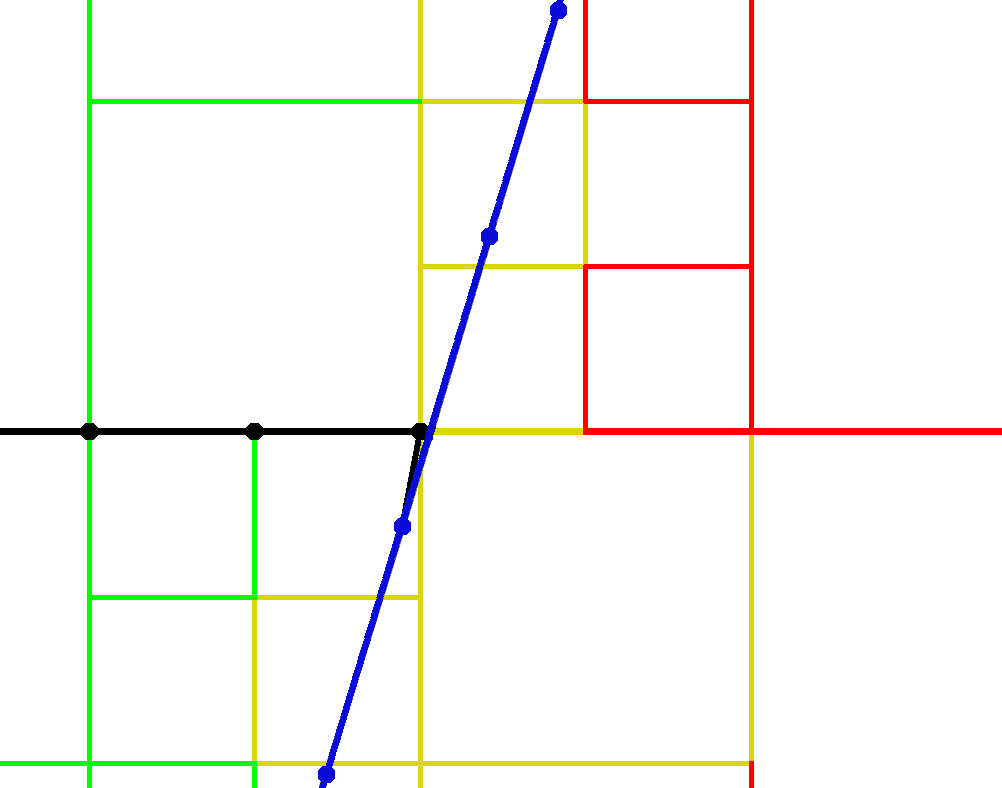
\includegraphics[width=\textwidth]{fig/teste_prox_error.png}}\end{minipage}
	}
	\caption{Possíveis casos no teste de proximidade.}
	\label{fig:teste_prox}
\end{figure}


A busca pelo vértice da fronteira mais próximo que intercepta a partição não garante a qualidade do subdomínio criado, pois, dependendo do refinamento da entrada e do posicionamento do corte da partição, o melhor vértice pode ter uma posição ruim para gerar malha. Se estes casos não forem tratados, o algoritmo de geração da malha possivelmente falhará ou gerará elementos de baixa qualidade.

Para tratar os casos citados, foram implementados testes de proximidade que utilizam as informações das células da estrutura de estimativa de carga. Com esses testes a qualidade da malha melhora além de se evitar possíveis erros na geração da malha.

O teste de proximidade é realizado quando a partição que está sendo criada utiliza uma célula da estrutura de estimativa de carga que intercepta a fronteira de entrada. Se isto ocorrer, será feita uma verificação se a célula da estrutura de estimativa de carga que está sendo testada é classificada como \textbf{sobre} a fronteira do domínio. Em caso afirmativo, será realizada uma busca pelo melhor vértice da fronteira que faz o maior angulo (Figura \ref{fig:teste_prox2}, onde entre as arestas $a$ e $c$, a melhor será $a$). Se o comprimento desta aresta for menor que o lado $b$ da célula da estrutura estimativa de carga que está sendo utilizada, será gerada a aresta que liga os dois vértices (Figura \ref{fig:teste_prox_fim}). Caso contrário, será criado um novo vértice segundo as informações da grade de suporte.

Esse teste é baseado na ideia de que para um bom elemento ser gerado ele precisa de uma área mínima. Neste trabalho é assumido que esta distância mínima deve ser o tamanho da célula da \textit{quadtree} de estimativa de carga para o caso bidimensional. Com este teste evita-se a criação de arestas com ângulos muito pequenos (Figura \ref{fig:teste_prox_error}) e melhora a qualidade dos elementos que serão gerados.

Esse mesmo teste se aplica a outros casos; um deles é quando a célula da partição tem uma região da sua célula tangente à fronteira de entrada, como mostrado na esquerda da Figura~\ref{fig:teste_prox_passos2}. Neste caso o teste de proximidade será efetuado várias vezes de tal forma que a medida que as arestas vão entrando no teste de proximidade, a região que está muito próxima da borda é transferida para a partição vizinha. Como consequência disso, parte da malha que seria gerada por um processador, será agora tratada pelo vizinho.


\begin{figure}[!ht]
	\centering
	\subfloat[Célula da estrutura de particionamento (em vermelho) juntamente com a borda de entrada.]
	{\label{fig:teste_prox_passos1}
		\begin{minipage}[c]{0.35\textwidth}{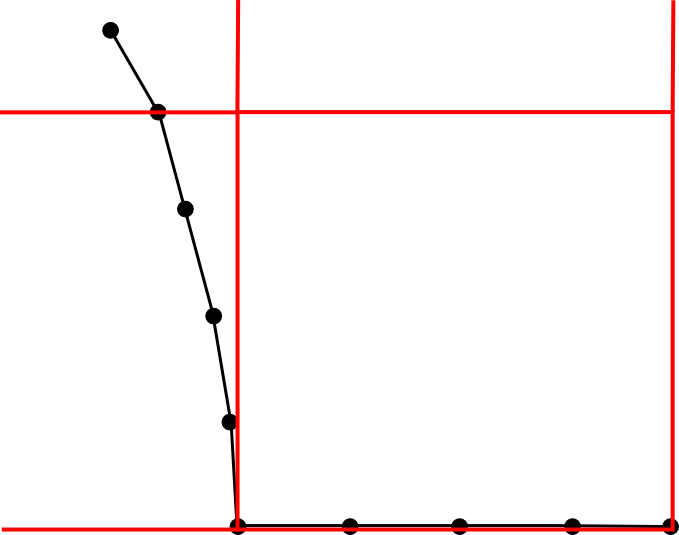
\includegraphics[width=\textwidth]{fig/prox_1.png}}\end{minipage}
	}
	\qquad
	\subfloat[Arestas em azul entram no teste de proximidade.]
	{\label{fig:teste_prox_passos2}
		\begin{minipage}[c]{0.35\textwidth}{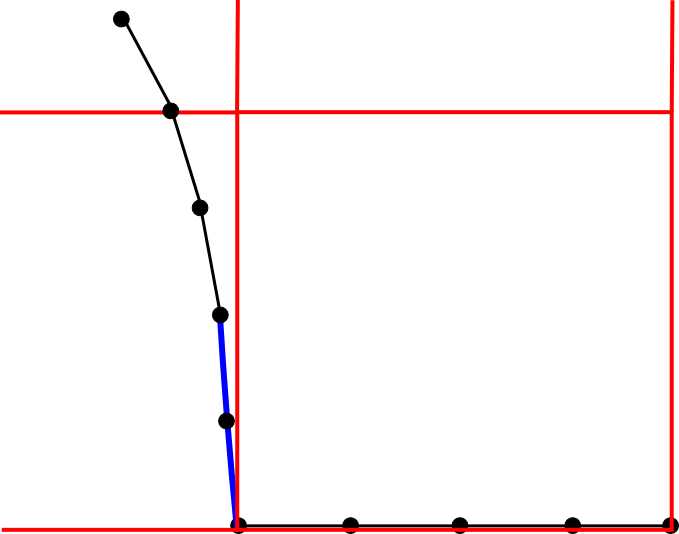
\includegraphics[width=\textwidth]{fig/prox_2.png}}\end{minipage}
	}    
	
	\subfloat[Após o teste de proximidade ser aplicado, o subdomínio azul fica responsável pela região onde as arestas falharam nos testes.]
	{\label{fig:teste_prox_passos3}
		\begin{minipage}[c]{0.35\textwidth}{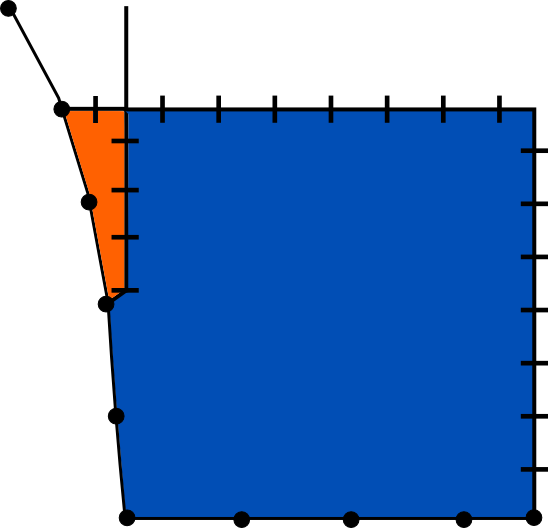
\includegraphics[width=\textwidth]{fig/prox_3.png}}\end{minipage}
	}    
	\qquad
	\subfloat[Subdomínios que seriam gerados sem a realização dos testes de proximidade.]
	{\label{fig:teste_prox_passos4}
		\begin{minipage}[c]{0.35\textwidth}{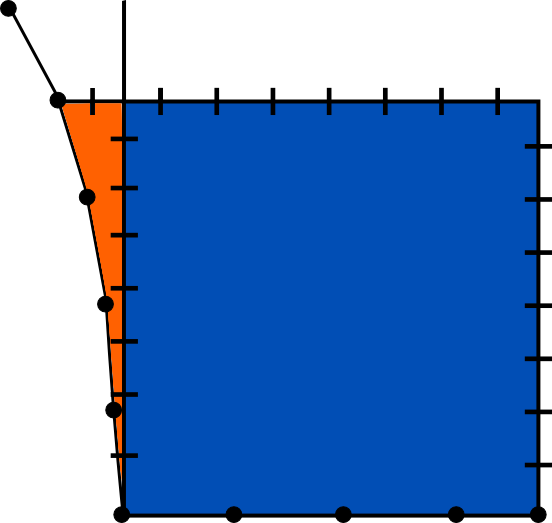
\includegraphics[width=\textwidth]{fig/prox_4.png}}\end{minipage}
	}    
	\caption{Modificações nas regiões realizadas pelo teste de proximidade para evitar elementos ruins.}
	\label{fig:teste_prox_passos}
\end{figure}


\subsubsection{Tratamento de Buracos}
\label{sec:Tratamento_buracos}

Alguns modelos possuem buracos em seus domínios, e, nesses casos, é preciso realizar um teste simples para evitar que sejam criadas arestas que atravessem a fronteira. Esse tratamento é realizado apenas quando uma partição da BSP intercepta algum buraco do modelo.

Quando se tem um buraco que intercepta a partição que está sendo criada, existirão células classificadas como fora da partição entre as que estão classificadas como dentro ou que cruzam a fronteira. O algoritmo tentará gerar uma aresta entre duas células classificadas como internas, mas essa aresta irá cruzar células classificadas como externas ao domínio. 

\begin{figure}[!ht]
	\centering
	\subfloat[Célula da estrutura de particionamento (em vermelho) juntamente com a borda de entrada que contém um buraco.]
	{\label{fig:teste_prox_buraco_passos1}
		\begin{minipage}[c]{0.35\textwidth}{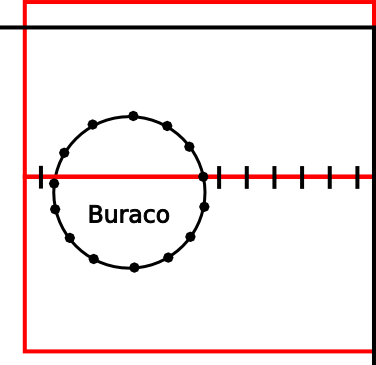
\includegraphics[width=\textwidth]{fig/buraco_1.png}}\end{minipage}
	}
	\qquad
	\subfloat[Detecta-se que arestas que seria criada de $a$ para $b$ passa por um buraco.]
	{\label{fig:teste_prox_buraco_passos2}
		\begin{minipage}[c]{0.35\textwidth}{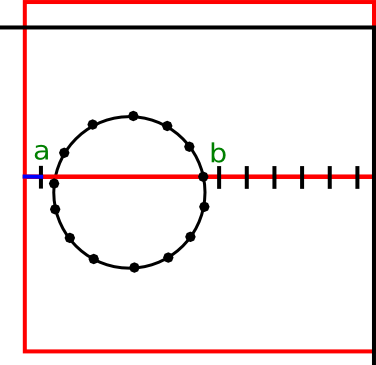
\includegraphics[width=\textwidth]{fig/buraco_2.png}}\end{minipage}
	}    
	\caption{Passos feitos nos tratamentos de buracos.}
	\label{fig:teste_prox_buraco_passos}
\end{figure}

\begin{figure}[!ht]
	\ContinuedFloat
	\centering    
	\subfloat[Teste feito para selecionar a melhor aresta para $a$.]
	{\label{fig:teste_prox_buraco_passos3}
		\begin{minipage}[c]{0.35\textwidth}{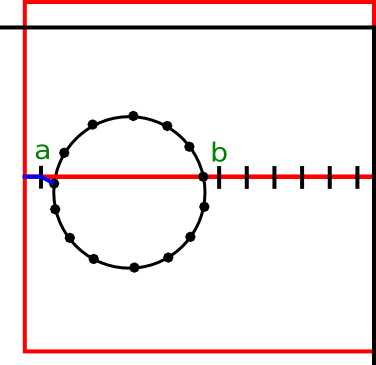
\includegraphics[width=\textwidth]{fig/buraco_3.png}}\end{minipage}
	}    
	\qquad
	\subfloat[Teste feito para selecionar a melhor aresta para $b$.]
	{\label{fig:teste_prox_buraco_passos4}
		\begin{minipage}[c]{0.35\textwidth}{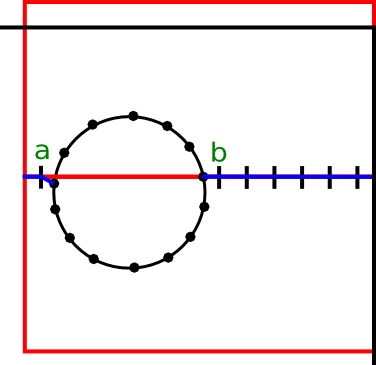
\includegraphics[width=\textwidth]{fig/buraco_4.png}}\end{minipage}
	}    
	\caption{Passos feitos nos tratamentos de buracos (continuação).}
\end{figure}

Quando é detectada uma possível colisão de uma aresta com células externas, serão criadas duas arestas em vez de uma. A primeira conecta o último vértice criado ao vértice mais próximo da primeira interseção do buraco com a partição da BSP (Figura \ref{fig:teste_prox_buraco_passos3}), e a segunda liga o vértice mais próximo da segunda interseção com o buraco a um vértice que será criado de acordo com a grade de suporte (Figura \ref{fig:teste_prox_buraco_passos4}).

\subsection{Geração da Interface Tridimensional}

???

\section{Balanceamento da Carga}


Após todos os subdomínios estarem devidamente criados, eles devem ser distribuídos entre os processadores disponíveis para que as submalhas sejam geradas por alguma técnica de geração de malha. Essa distribuição das tarefas deve ser feita de tal forma que todos os processadores gastem a mesma quantidade de tempo, evitando que algum processador fique sobrecarregado ou ocioso.

De acordo com o modo que o domínio é particionado, pode-se ter como resultado diversas tarefas para serem distribuídas (caso o número de tarefas seja maior que o de processadores) ou então ter a mesma quantidade de tarefas e processadores. O número de tarefas é o mesmo de folhas da BSP de particionamento, por isso uma estratégia de balanceamento não-centralizado que utiliza uma BSP para balancear a carga é utilizada neste trabalho.

O balanceamento de carga é feito a medida que novos cortes são feitos domínio. Inicialmente um único processador é responsável por realizar o primeiro corte, após isso, novos processadores irão sendo ativados para continuar o particionamento. Ao final do particionamento todos os processadores já estarão com os seus respectivos subdomínios. A Figura \ref{fig:arvore_balanceamento} mostra a árvore resultante para o balanceamento do modelo da Figura \ref{fig:celulas_selecionadas2d}.


\begin{figure}[!ht]
	\centering
	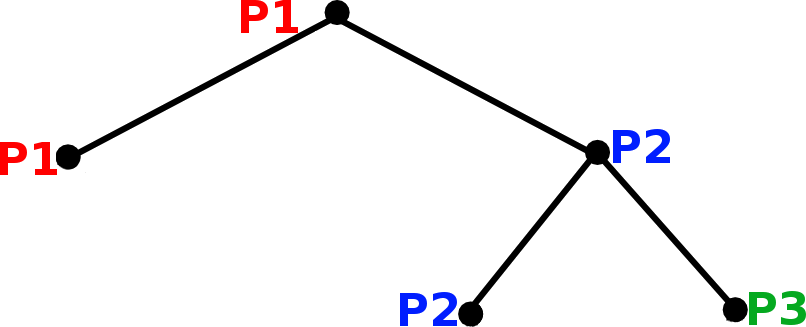
\includegraphics[width=0.5\textwidth]{fig/arvore_balanceamento.png}
	\caption{Balanceamento de carga feito para o modelo da Figura \ref{fig:celulas_selecionadas2d}.}
	\label{fig:arvore_balanceamento}
\end{figure}


Se a quantidade de tarefas e processadores forem iguais, cada processador receberá uma única tarefa, onde cada tarefa corresponde a uma célula folha da BSP de particionamento. Quando duas células que pertencem a um mesmo nó terminarem de fazer sua computação, um dos processadores dessas células ficará responsável por juntar as duas submalhas e fazer a melhoria na malha resultante. Esse processo é feito para cada par de células que pertence a um mesmo nó da BSP até chegar no nó raiz. A Figura \ref{fig:balanceamento_esfera} ilustra este processo.


\begin{figure}[!ht]
	\centering    
	\subfloat[Processador $P1$ será o responsável por fazer a junção da malha vermelha e azul.]
	{\label{fig:balanceamento_esfera1}
		\begin{minipage}[c]{0.3\textwidth}{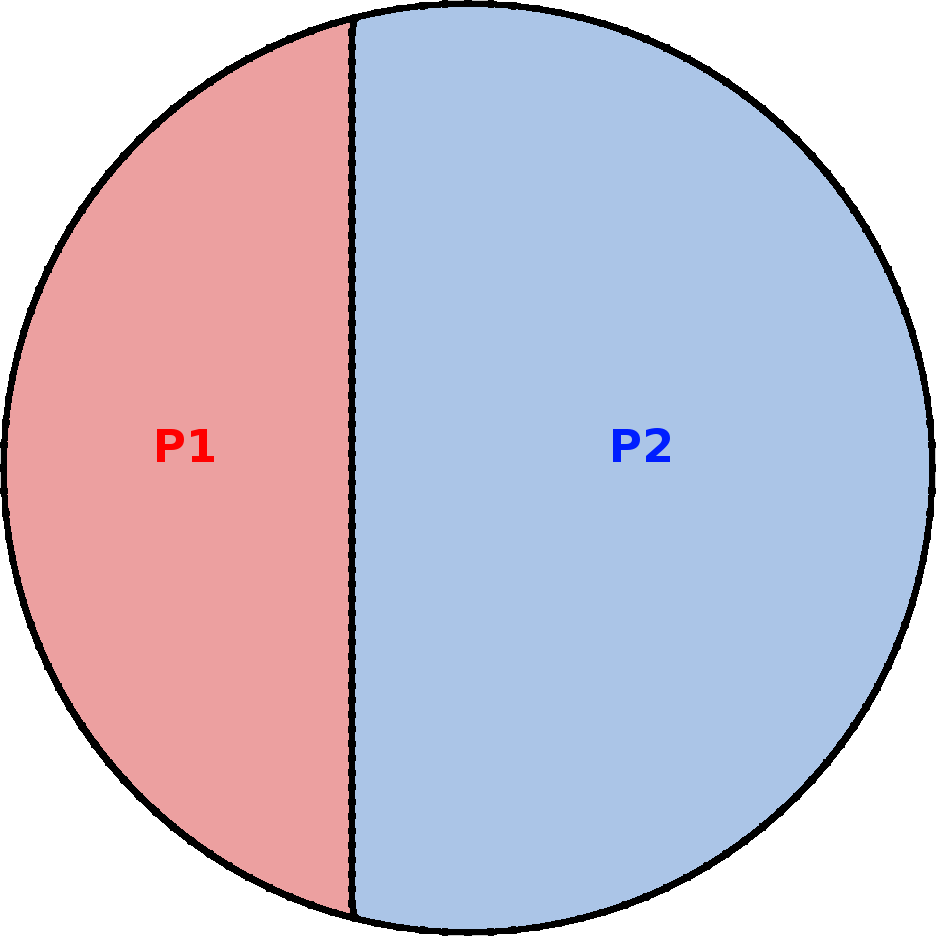
\includegraphics[width=\textwidth]{fig/balanceamento1.png}}\end{minipage}
	}
	\qquad
	\subfloat[Processador $P2$ será o responsável por fazer a junção da malha azul e verde.]
	{\label{fig:balanceamento_esfera2}
		\begin{minipage}[c]{0.3\textwidth}{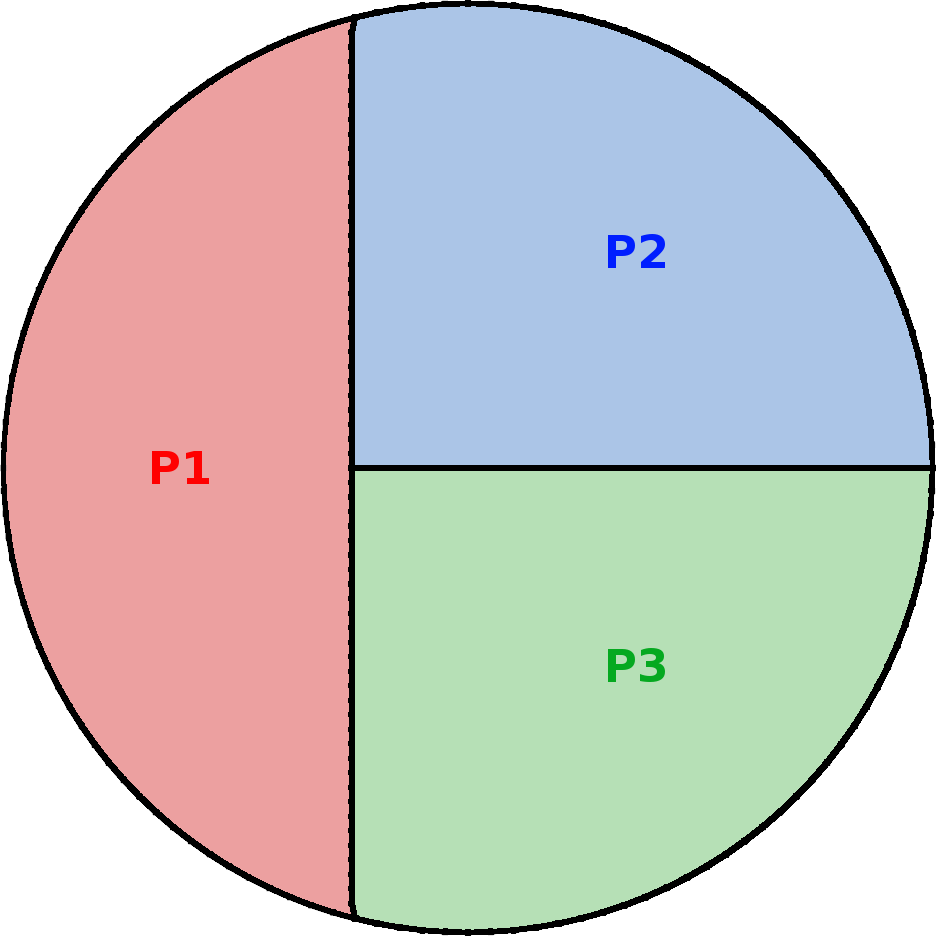
\includegraphics[width=\textwidth]{fig/balanceamento2.png}}\end{minipage}
	}
	\caption{Etapas do balanceamento de tarefas entre os processadores para o moledo da Figura \ref{fig:celulas_selecionadas2d}.}
	\label{fig:balanceamento_esfera}
\end{figure}


\section{Geração da Malha}

Cada processador tem a possibilidade de aplicar algoritmos diferentes se desejado, podendo se aplicado qualquer técnica de geração de malha que respeite os pré-requisitos citados no início deste capítulo. Foi selecionado uma técnica de Avanço de Fronteira para realizar os testes.

O algoritmo de Avanço de Fronteira utilizado foi desenvolvido em \cite{bib:Miranda99} e \cite{bib:Cavalcante-Neto01}. Foram utilizadas estruturas de dados geométricas para acelerar a busca por vértices candidatos para a geração de um novo triângulo e para a busca de possíveis arestas intersectantes, garantindo uma rápida execução do procedimento de geração de malha.

O processo de geração de malha consiste em três etapas. A primeira é baseada na geometria, tentando gerar elementos de boa qualidade mantendo a validade da malha. A segunda é baseada na topologia, buscando apenas gerar elementos válidos, mesmo eles não sendo de boa qualidade. A ultima fase é a de geração por retrocesso (\textit{back-tracking}), que tenta finalizar a geração da malha nas áreas onde não foi possível realizar o avanço de fronteira. Vale lembrar que nos casos tridimensionais nem sempre existe uma solução para a geração da malha.

Na versão bidimensional da técnica as duas primeiras fases são suficientes para gerar a malha triangular. Na versão tridimensional nem sempre as duas primeiras fases conseguem finalizar a malha, por isso é necessário o passo de geração por retrocesso (\textit{back-tracking}). A Figura \ref{fig:melhoria_arestas_faces} ilustra o processo de retrocesso aplicado a uma cavidade.


\begin{figure}[ht]
	\centering
	\subfloat[Cavidade em cinza.]
	{\label{fig:melhoria_arestas_faces_ruim1}
		\begin{minipage}[c]{0.25\textwidth}{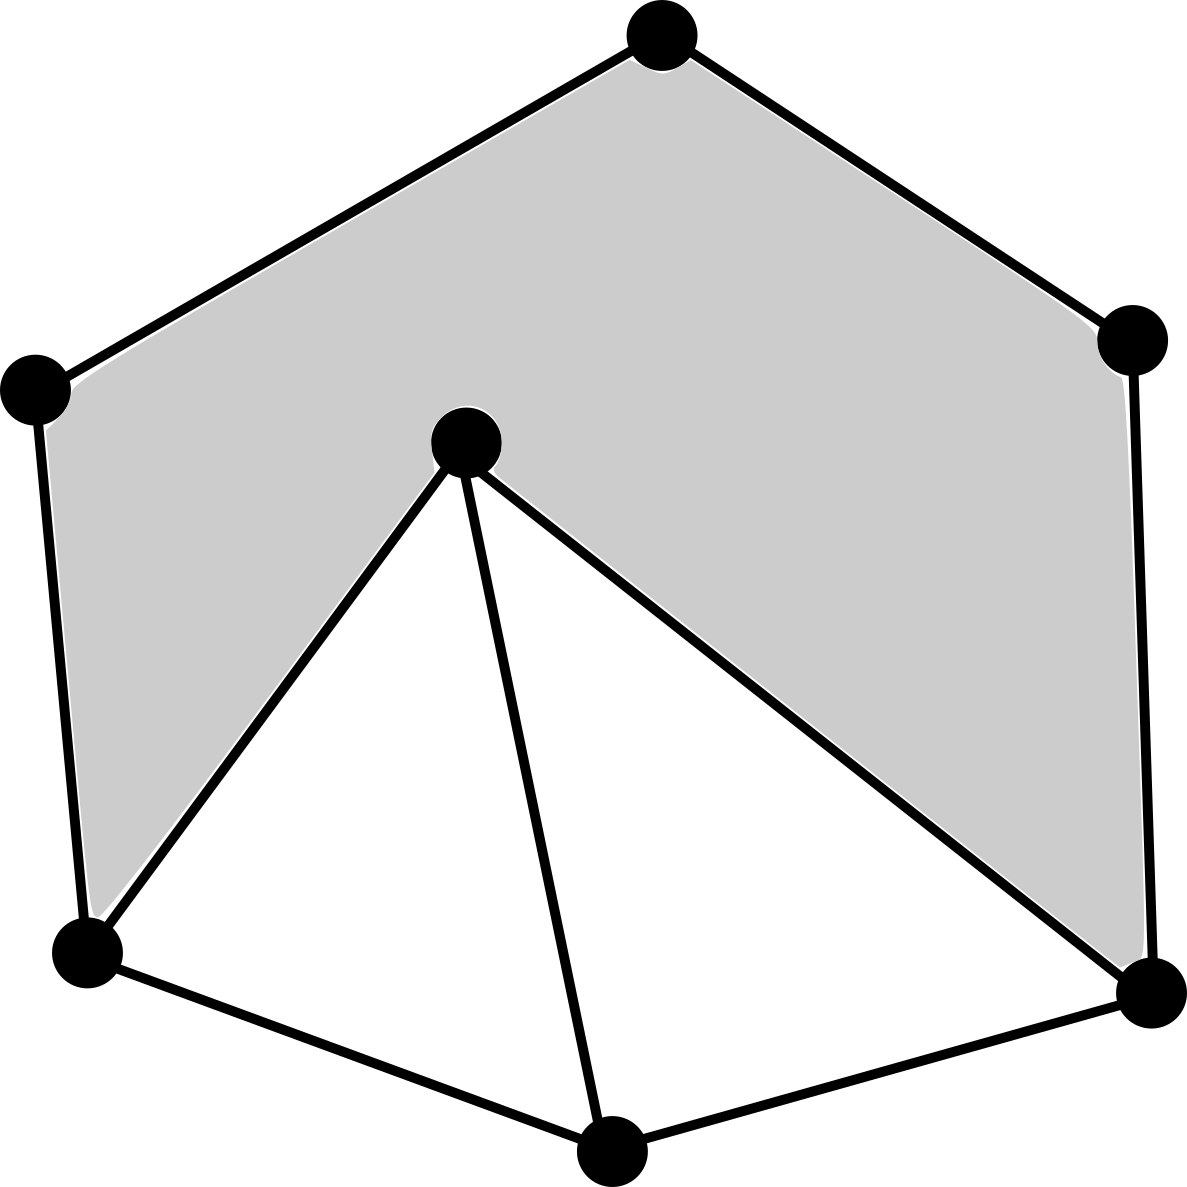
\includegraphics[width=\textwidth]{fig/backtracking1.png}}\end{minipage}
	}
	\qquad
	\subfloat[Teste de visibilidade sendo feito com o centroide (em azul) e suas arestas de teste.]
	{\label{fig:melhoria_arestas_faces_bom1}
		\begin{minipage}[c]{0.25\textwidth}{\includegraphics[width=\textwidth]{fig/backtracking2.png}}\end{minipage}
	}
	
	\subfloat[Cavidade após remoção de um elemento.]
	{\label{fig:melhoria_arestas_faces_ruim2}
		\begin{minipage}[c]{0.25\textwidth}{\includegraphics[width=\textwidth]{fig/backtracking3.png}}\end{minipage}
	}    
	\qquad
	\subfloat[Malha final, ligada ao centroide, após o retrocesso ser aplicado.]
	{\label{fig:melhoria_arestas_faces_bom2}
		\begin{minipage}[c]{0.25\textwidth}{\includegraphics[width=\textwidth]{fig/backtracking4.png}}\end{minipage}
	}
	\caption{Geração de malhas por retrocesso.}
	\label{fig:melhoria_arestas_faces}
\end{figure}


O processo de geração de malha é complementado com algumas melhorias. Ao todo são três etapas de melhorias, duas delas são modificações na topologia e a outra na geometria. As fases topológicas são a troca de faces (\textit{face swapping}) e a troca de arestas (\textit{edge swapping}), representadas nas Figuras \ref{fig:face_swapping} e \ref{fig:edge_swapping} respectivamente.


\begin{figure}[!ht]
	
	\centering
	\subfloat[Tetraedros adjacentes à face (1, 2, 3).]
	{\label{fig:face_swapping2}
	\begin{minipage}[c]{0.35\textwidth}\centering\includegraphics{fig/markos/face_swapping2.pdf}\end{minipage}}	
	\qquad	
	\subfloat[Tetraedros após a troca de faces ser realizada.]
	{\label{fig:face_swapping3}
	\begin{minipage}[c]{0.35\textwidth}\centering\includegraphics{fig/markos/face_swapping3.pdf}\end{minipage}}
	
	\caption{Troca de faces.}
	
	\label{fig:face_swapping}
	
\end{figure}


\begin{figure}[!ht]
	
	\centering
	\subfloat[Tetraedros adjacentes à aresta (1, 2).]
	{\label{fig:edge_swapping2}
	\begin{minipage}[c]{0.35\textwidth}\centering\includegraphics[scale=1.3]{fig/markos/edge_swapping3.pdf}\end{minipage}}
	\qquad	
	\subfloat[Tetraedros após a troca.]
	{\label{fig:edge_swapping3}
	\begin{minipage}[c]{0.35\textwidth}\centering\includegraphics[scale=1.3]{fig/markos/edge_swapping4.pdf}\end{minipage}}	
	\caption{Troca de arestas, com três tetraedros adjacentes (caso inverso à troca de faces).}	
	\label{fig:edge_swapping}
	
\end{figure}


Na fase geométrica é aplicada uma suavização de Laplace, onde os vértices internos da malha são movidos caso os elementos suavizados sejam melhores que o pior elemento antes da suavização. Esta suavização consiste em mover um vértice interno da malha de tal forma que ele se aproxime do centroide do polígono definido pelos seus vértices adjacentes, seguindo a Equação \ref{eq:laplace}. 


\begin{equation}
X_V^{n+1} = X_V^{n} + \phi \frac{\sum_{i=1}^m (X_i^n - X_V^n)}{m}
\label{eq:laplace}
\end{equation}


Nessa equação, $X_V^{n}$ é a posição do vértice $V$ na iteração de suavização $n$, $m$ é o número de vértices adjacentes a $V$ por algum tetraedro. $i$ corresponde o i-ésimo vértice adjacente a $V$, $X_V^{n}$ é a posição do i-ésimo vértice adjacente a V na iteração de suavização $n$, e $\phi$ é o parâmetro de relaxamento, normalmente ajustado para um valor entre 0 e 1 (neste trabalho, o valor de $1$ foi utilizado para $\phi$). A Figura \ref{fig:laplace} ilustra como a suavização é feita para $\phi=1,0$.



\begin{figure}[!ht]
	\centering
	\subfloat[Polígono formado pelos vértices adjacentes a $V$ (em vermelho).]
	{\label{fig:laplace1}
		\begin{minipage}[c]{0.25\textwidth}{\includegraphics[width=\textwidth]{fig/laplace1.png}}\end{minipage}
	}
	\qquad
	\subfloat[Centroide do polígono em azul.]
	{\label{fig:laplace2}
		\begin{minipage}[c]{0.25\textwidth}{\includegraphics[width=\textwidth]{fig/laplace2.png}}\end{minipage}
	}
	\qquad	
	\subfloat[Resultado final da suavização de Laplace.]
	{\label{fig:laplace3}
		\begin{minipage}[c]{0.25\textwidth}{\includegraphics[width=\textwidth]{fig/laplace3.png}}\end{minipage}
	}    
	\caption{Suavização de Laplace feita para $\phi=1,0$.}
	\label{fig:laplace}
\end{figure}


\section{Junção e Finalização da Malha}


\section{Conclusão}
